\newpage
\section{Настройка справочников}

\subsection{Принципы заполнения справочников в \tmis}

Работа \tmis~строится на базе справочников. В системе сведено к минимуму количество программно заданных значений. Большая часть вариантов выбора берется из настраиваемых справочников, что обеспечивает большую гибкость системы.

Для просмотра и редактирования справочников необходимо в главном меню выбрать пункт \dm{Справочники} и далее выбрать соответствующую группу и название справочника. Группировка справочников в меню выполнена в соответствии с назначением справочников.

В \tmis~существует 2 основных вида справочников:
\begin{itemize}
 \item линейные;
 \item иерархические.
\end{itemize}

Рассмотрим подробнее принцип организации каждого из них.

Справочники линейной структуры представляют собой таблицу (Рисунок \ref{img_spr_org}). В левом нижнем углу окна отображается количество записей справочника. В правом нижнем углу – кнопки управления записями справочника.

\begin{figure}[ht]\centering
 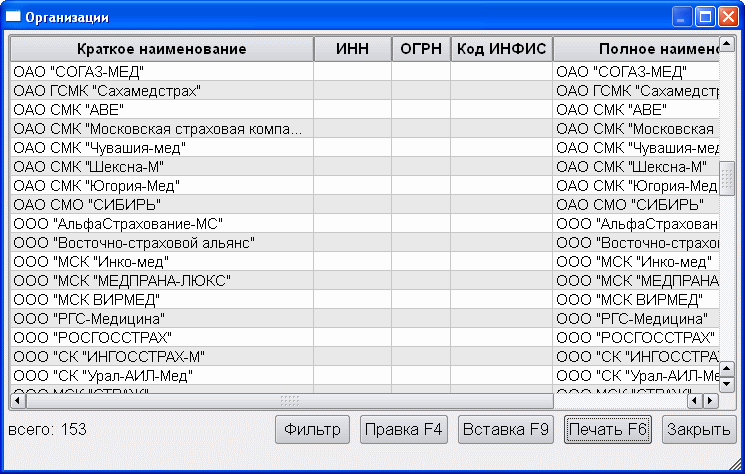
\includegraphics[width = 0.8\textwidth ,keepaspectratio]{spr_org}
 \caption{Пример линейной организации справочника}
 \label{img_spr_org}
\end{figure}

\begin{prim}
 В таблице при просмотре справочника могут отображаться не все его поля. Для просмотра подробной информации по каждой записи, необходимо установить на нее курсор и нажать кнопку \btn{Правка F4}  в нижней части окна.
\end{prim}
 
Для добавления записи в справочник нужно нажать кнопку \btn{Вставка F9} в нижней части окна или клавишу \keys{F9} на клавиатуре. Откроется карточка редактирования позиции справочника. Она может содержать от одного до десятков полей, при большом количестве полей, они могут быть разбиты на вкладки. 

Для редактирования записи из справочника нужно дважды щелкнуть по выбранной записи левой кнопкой мыши либо установить курсор на нужной записи и нажать кнопку \btn{Правка F4} в нижней части окна или клавишу \keys{F4} на клавиатуре. Откроется карточка редактирования позиции справочника. Следует внести в запись справочника необходимые изменения, а затем нажать кнопку \btn{OK}.

При нажатии на кнопку \btn{Печать F6} или клавишу \keys{F6} на клавиатуре открывается окно предварительного просмотра печатной формы справочника (Рисунок \ref{img_spr_prn}). Для отправки документа на принтер необходимо нажать кнопку \btn{Печатать}, для сохранения в файл – кнопку \btn{Сохранить}.

\begin{figure}[ht]\centering
 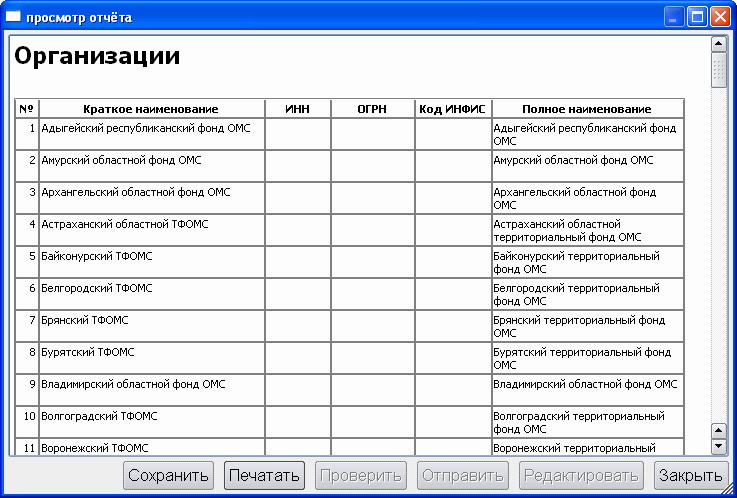
\includegraphics[width = 0.8\textwidth ,keepaspectratio]{spr_prn}
 \caption{Предварительный просмотр печати справочника}
 \label{img_spr_prn}
\end{figure}

Если справочник предполагает наличие большого числа записей, в окне редактирования справочника появляется дополнительная кнопка \btn{Фильтр}, при нажатии на которую открывается окно для задания параметров фильтрации (Рисунок \ref{img_spr_orgfnd}). Необходимо ввести условия отбора в поля и нажать кнопку \btn{OK}, после чего оно закроется, а на экране останутся только записи справочника, удовлетворяющие заданным условиям. Количество записей, указанное в левом нижнем углу окна, так же изменится и будет показывать количество записей, полученных в результате фильтрации. Состав и количество параметров фильтрации зависит от выбранного справочника.

\begin{figure}[ht!]\centering
 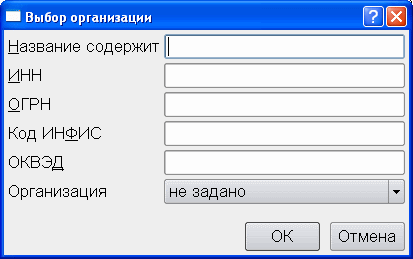
\includegraphics[width = 0.5\textwidth ,keepaspectratio]{spr_orgfnd}
 \caption{Окно параметров фильтрации записей справочника}
 \label{img_spr_orgfnd}
\end{figure}

В некоторых справочниках доступны дополнительные функции для работы с записями. Доступ к ним осуществляется через контекстное меню выбранной записи.

Иерархические справочники визуально разделены на 2 части: в левой части отображается справочник в виде дерева, в правой части отображаются дочерние элементы выбранной в левой части ветви дерева (Рисунок \ref{img_spr_str}). 

\begin{figure}[ht]\centering
 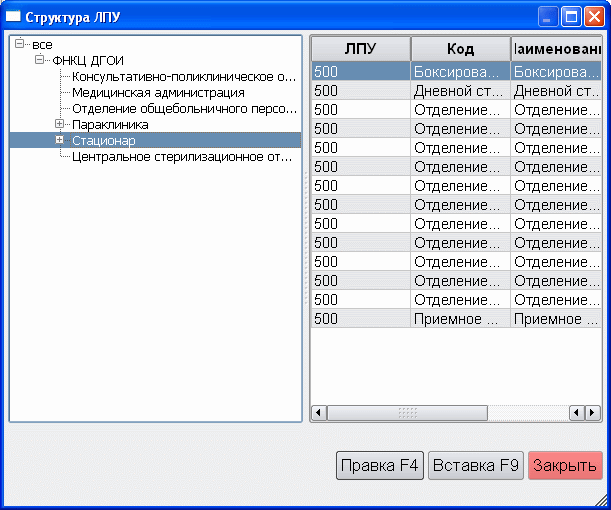
\includegraphics[width = 0.7\textwidth ,keepaspectratio]{spr_str}
 \caption{Пример справочника иерархической структуры}
 \label{img_spr_str}
\end{figure}

Кнопка \btn{Вставка F9}  позволяет добавить новый дочерний элемент в выбранную в левой части ветвь дерева. Кнопка \btn{Правка F4}  позволяет отредактировать выбранный в правой части окна дочерний элемент. Для изменения подчиненности элемента дерева нужно просто перетащить его в соответствующую группу с помощью мыши.

В зависимости от выбранного справочника, окно редактирования его элементов может содержать от одного до десятков полей. Каждый элемент может содержать в себе дополнительные таблицы, списки значений и т.п. Для просмотра всех полей элемента справочника необходимо открыть его на редактирование.

Для удаления записи из справочника следует щелкнуть правой кнопкой мыши по записи, подлежащей удалению, в правой части окна и в появившемся контекстном меню выбрать \dm{Удалить запись}.

\begin{vnim}
 Удаление элементов справочника, которые уже были использованы в системе, может привести к серьезным ошибкам. Такие элементы удалять крайне не рекомендуется. Будьте осторожны!
\end{vnim}

\subsection{Состав и назначение справочников \tmis}

В таблице 2 приведено описание и назначение всех справочников системы. Справочники, номера которых помечены символом <<*>> будут рассмотрены ниже более подробно.

{\small
\begin{longtable}{|p{0.55cm}|p{2.45cm}|p{5.65cm}|p{1.85cm}|p{1.95cm}|p{3.2cm}|}
\caption{Справочники \tmis \label{tbl_spr}}\\
\hline \rule{0pt}{15pt} \centering \textbf{N пп} & \centering \textbf{Название справочника} & \centering \textbf{Описание справочника} & \centering \textbf{Группа в меню} & \centering \textbf{Назна\-че-ние} & \textbf{Зависимости}\\ \hline
\endfirsthead
\hline \rule{0pt}{15pt} \centering \textbf{N пп} & \centering \textbf{Название справочника} & \centering \textbf{Описание справочника} & \centering \textbf{Группа в меню} & \centering \textbf{Назначе-ние} & \textbf{Зависимости}\\ \hline
\endhead
1 & Воинские части	& &	Адреса	& &	Нет зависимостей \\ \hline
2* & Структура ЛПУ	& Описание структуры ЛПУ в виде иерархического справочника. Записи справочника содержат подробную информацию о подразделении на нескольких вкладках, в том числе информацию о зоне обслуживания, видах выполняемых работ, койках (для отделения стационара) и т.п. Данный справочник используется во всех действиях системы, где необходимо указать подразделение ЛПУ & Персонал & Базовый	& \textbf{Требуются справочники}: Организации, Сеть (взрослая\slash детская\slash женская), Типы событий; \textbf{Опционально}: Типы действий, Профили коек, Типы работ, Специальности, Сотрудники. \\ \hline
3 &	Виды деятельности &	Справочник видов деятельности для сотрудников. Возможна фильтрация сотрудников по виду деятельности на панели \dm{График} &	Персонал & Сотруд\-ни\-ки	& Нет зависимостей \\ \hline
4 &	Должности	& Справочник должностей для сотрудников, используется для указания должностей сотрудников в справочнике \dm{Сотрудники} &	Персонал & 	Сотруд\-ни\-ки	& Нет зависимостей \\ \hline
5 &	Специаль\-нос\-ти &	Справочник специальностей сотрудников, используется для регистрации специальности сотрудников в справочнике Сотрудники. Возможна фильтрация и получение отчетов по специальности врача & Персонал &	Сотруд\-ни\-ки &	Нет зависимостей \\ \hline
6* & Сотрудники & Список сотрудников ЛПУ, является одновременно справочником пользователей \tmis. Содержит данные кадрового учета о сотруднике, его квалификации, графике работы, учетные данные для входа пользователя в систему и т.д. Выбор врача или исполнителя во всех действиях в системе производится из данного справочника. & Персонал & 	Базовый & \textbf{Требуются справочники}: Организации, Должности, Специальности, Ученые степени, Ученые звания, Структура ЛПУ; \textbf{Опционально}: Виды деятельности, Роли пользователей, Тип документа, Источники финансирования \\ \hline
7 &	Ученые звания	& Справочник используется для указания ученых званий сотрудников в справочнике \dm{Сотрудники}	& Персонал	& Сотруд\-ни\-ки	& Нет зависимостей \\ \hline
8 &	Ученые степени &	Справочник используется для указания ученых степеней сотрудников в справочнике \dm{Сотрудники}	& Персонал &	Сотруд\-ни\-ки &	Нет зависимостей \\ \hline
9 &	Коды МКБ Х &	Справочник необходим при регистрации диагнозов пациента по классификатору МКБ-10 &	Медицинс\-кие & Лечебный процесс	& Нет обязательных зависимостей; \textbf{Опционально}: Услуга (профиль ЕИС) \\ \hline
10 & 	Субклассифи\-кация МКБ по пятому знаку &	Справочник локализаций заболеваний необходим при регистрации диагнозов пациента по классификатору МКБ-10 с точностью до 5-го знака & Медицинс\-кие &	Лечебный процесс &	Нет зависимостей \\ \hline
11 &	Характеры заболеваний &	Характер течения заболевания (острое, хроническое и т.п.), используется при регистрации диагнозов пациентов	 & Медицинс\-кие	& Лечебный процесс	& Нет зависимостей \\ \hline
12	& Стадии заболеваний & (Основной, сопутствующий, осложнение), используется при регистрации диагнозов пациентов	& Медицинс\-кие &	Лечебный процесс	& Нет зависимостей \\ \hline
13	& Типы диагноза &	Используется при регистрации диагнозов пациентов &	Медицинс\-кие &	Лечебный процесс	& Нет зависимостей \\ \hline
14	& Типы травмы	& Используется при регистрации диагнозов пациентов &	Медицинс\-кие	& Лечебный процесс	& Нет зависимостей \\ \hline
15	& Группы здоровья	& Используется при регистрации диагнозов пациентов &	Медицинс\-кие	& Лечебный процесс	& Нет зависимостей \\ \hline
16	& Отметки диспансерного наблюдения &	Используется при регистрации диагнозов пациентов	& Медицинс\-кие	& Лечебный процесс	& Нет зависимостей \\ \hline
17 &	Результаты осмотра &	Результаты обращений пациентов настраиваются отдельно для каждой цели визита, указывается при закрытии обращений &	Медицинс\-кие	& Лечебный процесс &	\textbf{Требуется справочник}: Назначение типа события \\ \hline
18	& Причины ВУТ, инвалидности или ограничения жизнедеятельности &	На данный момент не используется. Функционал находится в разработке	 & Медицинс\-кие	& ВУТ	& Нет зависимостей \\ \hline
19 &	Документы ВУТ, инвалидности или ограничения жизнедеятельности &	На данный момент не используется. Функционал находится в разработке	& Медицинс\-кие &	ВУТ	& Нет зависимостей \\ \hline
20 &	Режимы периода ВУТ, инвалидности или ограничения жизнедеятельности &	На данный момент не используется. Функционал находится в разработке	& Медицинс\-кие &	ВУТ &	Нет зависимостей \\ \hline
21 & Нарушения режима ВУТ &	На данный момент не используется. Функционал находится в разработке	& Медицинс\-кие &	ВУТ &	Нет зависимостей \\ \hline
22 & Результаты периода ВУТ, инвалидности или ограничения жизнедеятельности &	На данный момент не используется. Функционал находится в разработке	& Медицинс\-кие	& ВУТ	& Нет зависимостей \\ \hline
23 &	Причины выдачи дубликатов документов ВУТ &	На данный момент не используется. Функционал находится в разработке	& Медицинс\-кие	& ВУТ	& Нет зависимостей \\ \hline
24	& Жалобы &	Справочник жалоб пациентов, используется при предварительной записи на прием или вызове врача на дом, а так же при заполнении свойства \dm{Жалобы} действий	& Медицинс\-кие &	Поликли\-ни\-ка &	Нет зависимостей \\ \hline
25 & Тезаурус &	Иерархический справочник  стандартных фраз для заполнения свойств действий. Возможность использования данного справочника для определенного свойства настраивается в справочнике \dm{Типы действий}, при этом возможно использование отдельных ветвей дерева различных уровней иерархии	 & Медицинс\-кие &	Лечебный процесс &	Нет зависимостей \\ \hline
26 &	Группы крови	& Справочник используется для указания группы крови пациента в его регистрационной карточке &	Медицинс\-кие &	Регистра\-ция пациентов &	Нет зависимостей \\ \hline
27 &	Фазы заболеваний &	Используется при регистрации диагнозов пациентов	& Медицинс\-кие &	Лечебный процесс	& Нет зависимостей \\ \hline
28 &	Отметки проблемных зон &	Справочник изображений для нанесения маркеров. Используется для нанесения меток на графическое изображение в свойствах действий. При регистрации новой записи справочника необходимо загрузить изображение, которое будет являться фоном для нанесения маркеров (например, схематическое изображение тела человека) и задать размер маркеров. Возможность использования данного справочника в работе пользователей настраивается в справочнике \dm{Типы действий} & Медицинс\-кие	& Лечебный процесс	& Нет зависимостей \\ \hline
29 &	Типы операций &	Справочник значений свойства действий типа OperationType. Возможность использования данного справочника в работе пользователей настраивается в справочнике \dm{Типы действий} &	Медицинс\-кие &	Лечебный процесс	& \textbf{Опционально:} Категории операций \\ \hline
30 &	Категории операций &	Справочник категорий для справочника \dm{Типы операций} &	Медицинс\-кие &	Лечебный процесс	& Нет зависимостей \\ \hline
31	& Модели пациента	& Используется при регистрации талона ВМП	& Медицинс\-кие	& ВМП &	\textbf{Требуется справочник}: Виды квот \\ \hline
32 &	Методы лечения	& Используется при регистрации талона ВМП	& Медицинс\-кие	& ВМП & 	\textbf{Требуется справочник}: Модели пациента \\ \hline
33 &	Связи МКБ-Модель пациента -~ Тип квоты &	Используется при регистрации талона ВМП	& Медицинс\-кие	& ВМП &	\textbf{Требуются справочники}: Модели пациента, Виды квот, Методы лечения \\ \hline
34 &	Исходы заболеваний &	Регистрация исхода в обращениях. Исход обращения задается в зависимости от цели обращения (назначения типа события) &	Медицинс\-кие	& Лечебный процесс & 	\textbf{Требуется справочник}: Назначение типа события \\ \hline
35 &	ОКПФ (организаци\-онно-правовая форма)	& Используется при регистрации организаций & 	Класси\-фи\-ка\-то\-ры &	Органи\-за\-ции	& Нет зависимостей \\ \hline
36 &	ОКФС (форма собственности) &	Используется при регистрации организаций &	Класси\-фи\-ка\-то\-ры &	Органи\-за\-ции	& Нет зависимостей \\ \hline
37 &	Типы вредности &	Регистрация профессиональных вредностей в регистрационной карточке пациента 	& Класси\-фи\-ка\-то\-ры &	Регистра\-ция пациентов &	Нет зависимостей \\ \hline
38	& Факторы вредности &	Регистрация факторов вредности в регистрационной карточке пациента & 	Класси\-фи\-ка\-то\-ры &	Регистра\-ция пациентов	& Нет зависимостей \\ \hline
39	& Единицы измерения	& Единицы измерения для результатов лабораторных исследований & 	Класси\-фи\-ка\-то\-ры	& Лаборато\-рия	& Нет зависимостей \\ \hline
40	& Место выполнения визита	& Может быть задано для каждого типа события. Для поликлинических обращений место посещения выбирается из данного справочника & Учет	& Лечебный процесс	& Нет зависимостей \\ \hline
41 & Типы визитов	& Задается тип посещения для поликлинических типов обращений & Учет &	Лечебный процесс &	Нет зависимостей \\ \hline
42 &	Библиотека свойств действий &	Записи из библиотеки могут быть использованы в качестве шаблонов при добавлении свойств в типы действий (на данный момент переносится только наименование) &	Учет	& Лечебный процесс &	\textbf{Требуется справочник}: Услуга (профиль ЕИС) \\ \hline
43	& Шаблоны действий & 	Справочник предназначен для просмотра и редактирования сохраненных пользователями шаблонов. Отдельное заполнение его не требуется. Как правило, он наполняется в процессе работы системы	& Учет &	Печатные формы &	Нет зависимостей \\ \hline
44 & Графики выполнения назначений	& Варианты стандартных схем выполнения назначений (как правило, медикаментозных). Указывается время выполнения назначения в течении суток, можно указать несколько периодов выполнения	& Учет &	Стацио\-нар &	Нет зависимостей \\ \hline
45* &	Типы действий &	Задается описание типов действий, настраивается их внешний вид, состав свойств действий, соответствие услуги в зависимости от источника финансирования, проверки и т.п. &	Учет	& Базовый	& \textbf{Требуются справочники (опционально)}: Сотрудники, Типы работ, Единицы измерения, Виды квот, Услуга (профиль ЕИС), Тип ткани, Источники финансирования \\ \hline
46* &	Табличные свойства типов действий &	Получение таблиц значений для свойств действий из различных таблиц БД & Учет &	Лечебный процесс &	Нет зависимостей \\ \hline
47	& Типы медицинской помощи &	Дополнительная, более детальная, классификация типов событий &	Учет &	Лечебный процесс &	Нет зависимостей \\ \hline
48	& Категории медицинской помощи	& Категории медицинской помощи для типов событий &	Учет &	Лечебный процесс	& Нет зависимостей \\ \hline
49	& Профили медицинской помощи	& Профили медицинской помощи, использующиеся при выставлении счетов на оплату услуг &	Учет &	Финансо\-во-эконо\-ми\-чеcкий блок	& Нет зависимостей \\ \hline
50 &	Назначение типа события &	Используется в других справочниках для распределения групп значений по типам событий &	Учет	& Лечебный процесс &	Нет зависимостей \\ \hline
51	& Профили событий	& 	& Учет	& Лечебный процесс &	Нет зависимостей \\ \hline
52* &	Типы событий	& Настройка типов событий, использующихся в системе. Информация содержится на нескольких вкладках	& Учет	& Базовый	& \textbf{Требуются справочники}: Назначение типа события, Профили событий, Типы медицинской помощи, Категории медицинской помощи, Типы обращений, Источники финансирования; опционально: Услуга (профиль ЕИС), Место выполнения визитов, Типы визитов, Специальности, Группы здоровья, Отметки диспансерного наблюдения, Типы визитов, Типы действий. \\ \hline
53* &	Типы обращений	& Содержит список доступных типов обращений. Коды записей должны соответствовать приведенным в таблице 13 &
Учет	& Лечебный процесс &	Нет зависимостей \\ \hline
54	& Особенности выполнения МЭС	& Применяется при использовании МЭС для контроля лечебного процесса	& Учет &	МЭС &	Нет зависимостей \\ \hline
55	& Тип прикрепления	& Указывается в регистрационной карточке пациента, возможна фильтрация пациентов по данному признаку, составление отчетов	& Учет	& Регистра\-ция пациентов	& \textbf{Требуется справочник}: Источники финансирования \\ \hline
56	& Единицы учета медицинской помощи &	Единицы учета медицинской помощи для выставления счетов и оплаты &	Учет	& Финансо\-во-эконо\-мический блок &	Нет зависимостей \\ \hline
57	& Причины отсутствия	& Причины отсутствия сотрудников, используются в табеле рабочего времени	& Учет & Сотруд\-ни\-ки	& Нет зависимостей \\ \hline
58 &	Профили коек &	Используются при регистрации новых коек и размещении пациента в отделении	& Учет	& Стацио\-нар &	\textbf{Требуется справочник (опционально)}: Услуга (профиль ЕИС) \\ \hline
59* &	Типы работ &	Типы работ, выполняемые в системе	& Учет	& Базовый	& \textbf{Требуется справочник (опционально)}: Лабораторные информационные системы \\ \hline
60 &	Виды квот	& Виды квот для ВМП &	Учет &	ВМП	& Нет зависимостей \\ \hline
61	& Типы согласования	& Типы согласования для ВМП & 	Учет	& ВМП	& Нет зависимостей \\ \hline
62	& Типы бланков & Типы бланков строгой отчетности для регистрации нетрудоспособности пациента и пр.	& Учет	& ВУТ	& Нет зависимостей \\ \hline
63 &	Связь категории помощи и способа оплаты услуг	& Задает способы оплаты и тарифы для каждой категории медицинской помощи &	Учет	& Финансо\-во-эконо\-мический блок &	\textbf{Требуются справочники}: Категория помощи, Тип события, Единица учета помощи, Способы оплаты, Виды тарификации \\ \hline
64 &	Сеть (взрослая\slash детская\slash женская) &	Справочник видов ЛПУ по категориям обслуживаемого населения или типу помощи &	Организа\-ции &	Организа\-ции &	Нет зависимостей \\ \hline
65	& Банки	& Справочник банков для регистрации расчетных счетов организаций	& Организа\-ции & 	Финансо\-во-эконо\-мический блок	& Нет зависимостей \\ \hline
66* &	Организации &	В справочнике организаций необходимо регистрировать ЛПУ (в том числе базовое ЛПУ), СМО, организации-работодатели и др. В зависимости от указанного типа организация будет производиться фильтрация записей справочника при его использовании в различном контексте &	Организа\-ции	& Базовый	& \textbf{Требуются справочники}: Сеть (взрослая/детская/ женская); \textbf{Опционально}: Банки, ОКПФ (организа\-ци\-онно-правовая форма), ОКФС (форма собственности) \\ \hline 
67 & УФМС &	Справочник Управлений федеральной миграционной службы, позволяет выбрать из списка значение поля \dm{Выдан} документа, удостоверяющего личность пациента &	Организа\-ции	& Регистра\-ция пациентов & Нет зависимостей \\ \hline
68 & Источники финансирования	& Источник финансирования события указывается при регистрации обращения, используется при фильтрации и в отчетах &	Финансо\-вые &	Лечебный процесс &	Нет зависимостей \\ \hline
69 &	Услуга(про\-филь ЕИС)	& Каждое событие или действие, подлежащее оплате, должно быть связано с услугой. Только услуги можно выставить к оплате.	& Финансо\-вые	& Финансо\-во-эконо\-мический блок	&\textbf{Требуются справочники} (опционально): Категории медицинской помощи, Специальности, Профили медицинской помощи \\ \hline
70	& Тарифные категории	& & Финансо\-вые &	Финансо\-во-эконо\-мический блок &	Нет зависимостей \\ \hline
71	& Причины отказа платежа & Причины отказа при выставлении счетов СМО	& Финансо\-вые	& Финансо\-во-эконо\-мический блок	& Нет зависимостей \\ \hline
72	& Кассовые операции &	Виды кассовых операций &	Финансо\-вые &	Финансо\-во-эконо\-мический блок &	Нет зависимостей \\ \hline
73	& Источники финансирования услуг &	Источники финансирования, использующиеся при выставлении счетов на оплату услуг	& Финансо\-вые	& Финансо\-во-эконо\-мический блок	& Нет зависимостей \\ \hline
74	& Способы оплаты	& Используется в справочнике \dm{Связь категории помощи и способа оплаты услуг}	& Финансо\-вые	& Финансо\-во-эконо\-мический блок &	Нет зависимостей \\ \hline
75	& Виды тарификации	& Используется в справочнике \dm{Связь категории помощи и способа оплаты услуг}	& Финансо\-вые	& Финансо\-во-эконо\-мический блок &	Нет зависимостей \\ \hline
76	& Социальный статус: тип(льготы) &	Справочник значений социальных статусов &	Социаль\-ный статус	& Регистра\-ция пациентов	& Нет зависимостей \\ \hline
77	& Классифика\-тор социальных статусов &	Список классов социальных статусов. Для каждого класса при открытии на редактирование настраивается список доступных значений (см. п. 75) &	Социаль\-ный статус	& Регистра\-ция пациентов &	\textbf{Требуется справочник}: Социальный статус (тип льготы) \\ \hline
78* &	Тип полиса &	Тип полиса указывается при регистрации документов пациента. Коды типов полиса должны соответствовать приведенным в таблице 14 & Персони\-фикация	& Регистра\-ция пациентов	& Нет зависимостей \\ \hline
79*	& Группа типа документа (удостоверение, льготы и т.д.) &	Группировка документов по типу использования. Коды групп документов должны соответствовать указанным в таблице 16 &
Персони\-фикация	& Регистра\-ция пациентов	& Нет зависимостей \\ \hline
80	& Тип документа (паспорт и пр.)	& Тип документов указывается при регистрации персональных данных пациента	& Персони\-фикация	& Регистра\-ция пациентов	& \textbf{Требуется справочник}: Группа типа документа (удостоверение, льготы и т.п.) \\ \hline
81	& Различные способы связи с пациентом	& Типы способов связи (телефон, e-mail и т.п.)	& Персони\-фикация	& Регистра\-ция пациентов	& Нет зависимостей \\ \hline
82	& Типы связей пациента	& Типы родственных связей пациента. Родственные связи можно указать в регистрационной карточке пациента	& Персони\-фикация	& Регистра\-ция пациентов &	Нет зависимостей \\ \hline
83	& Бригады	& В данный момент не используется. Функционал находится в разработке. &	Скорая помощь &	Скорая помощь	& \textbf{Требуется справочник}: Сотрудники \\ \hline
84	& Повод к вызову & В данный момент не используется. Функционал находится в разработке. & Скорая помощь &	Скорая помощь	& Нет зависимостей \\ \hline
85	& Транспорти\-ровку перенес & В данный момент не используется. Функционал находится в разработке. & Скорая помощь & Скорая помощь &	Нет зависимостей \\ \hline
86	& Место получения вызова	& В данный момент не используется. Функционал находится в разработке. &	Скорая помощь	& Скорая помощь &	Нет зависимостей \\ \hline
87	& Вызов получен	& В данный момент не используется. Функционал находится в разработке. &	Скорая помощь &	Скорая помощь &	Нет зависимостей \\ \hline
88	& Причина задержки & В данный момент не используется. Функционал находится в разработке. &	Скорая помощь	& Скорая помощь	& Нет зависимостей \\ \hline
89	& Результат	& В данный момент не используется. Функционал находится в разработке. & Скорая помощь	& Скорая помощь	& Нет зависимостей \\ \hline
90	& Несчастный случай & В данный момент не используется. Функционал находится в разработке. &	Скорая помощь	& Скорая помощь	& Нет зависимостей \\ \hline
91	& Смерть	& В данный момент не используется. Функционал находится в разработке. & Скорая помощь	& Скорая помощь	& Нет зависимостей \\ \hline
92	& Опьянение	& В данный момент не используется. Функционал находится в разработке. &	Скорая помощь	& Скорая помощь	& Нет зависимостей \\ \hline
93	& Больной	& В данный момент не используется. Функционал находится в разработке. &	Скорая помощь	& Скорая помощь &	Нет зависимостей \\ \hline
94	& Место вызова & В данный момент не используется. Функционал находится в разработке. &	Скорая помощь	& Скорая помощь	& Нет зависимостей \\ \hline
95	& Способ транспортировки & В данный момент не используется. Функционал находится в разработке. &	Скорая помощь &	Скорая помощь &	Нет зависимостей \\ \hline
96	& Активное посещение	& В данный момент не используется. Функционал находится в разработке. &	Скорая помощь &	Скорая помощь &	Нет зависимостей \\ \hline
97	& Периоды питания	& Указывается время получения пищи	& Питание	& Питание в стационаре &	Нет зависимостей \\ \hline
98	& Столы питания	& Справочник видов столов	& Питание	& Питание в стационаре	& Нет зависимостей \\ \hline
99	& Шаблоны питания	& В данном справочнике осуществляется связь периодов питания и столов питания	& Питание	& Питание в стационаре	& \textbf{Требуются справочники}: Периоды питания, Столы питания \\ \hline
100	& Номенкла\-ту\-ра &	Справочник ЛС для назначений	& Лекарст\-венные средства и изделия медицинского назначения &	Стацио\-нар &	Нет зависимостей \\ \hline
101 &	Типы тканей	& Типы биоматериала для исследований	& Лаборато\-рия	& Лаборато\-рия	& Нет зависимостей \\ \hline
102	& Показатели исследований	& Коды и названия показателей исследований, передаваемые из ЛИС	& Лаборато\-рия	& Лаборато\-рия & Нет зависимостей \\ \hline
103	& Лаборатор\-ные информационные системы &	Настройка связи с ЛИС &	Лаборато\-рия	& Лаборато\-рия	& \textbf{Требуется справочник}: Показатели исследований \\ \hline
104	& Типы пробирок &	Типы пробирок и контейнеров, используемых в ЛИС	& Лаборато\-рия	& Лаборато\-рия	& \textbf{Требуется справочник}: Единицы измерения \\ \hline 
\end{longtable}
}

Справочники, для которых в поле <<Применение>> указано значение <<Базовый>>, являются обязательными для заполнения на этапе подготовки к внедрению. Без заполнения этих справочников работа \tmis~становится невозможной. Рекомендуется следующая последовательность заполнения указанных справочников:
\begin{enumerate}
 \item Организации. Как минимум, необходимо добавить в справочник информацию о базовом ЛПУ.
 \item Структура ЛПУ. На первоначальном этапе достаточно заполнить общую информацию о подразделении на вкладке \dm{Основная информация}. Информацию на остальных вкладках можно заполнять поэтапно (в соответствии с потребностями этапов внедрения).
 \item Сотрудники. Необходимо заполнить информацию о сотрудниках и пользователях системы
 \item Типы событий.
 \item Типы действий.
\end{enumerate}
 
Ниже будут рассмотрены особенности заполнения указанных и некоторых дополнительных справочников.

\subsection{Редактор плоских справочников}

Редактор плоских справочников позволяет создавать в \tmis~дополнительные справочники произвольной структуры. Редактор можно вызвать из главного меню \mm{Справочники \str Плоские справочники}. При этом откроется окно (Рисунок \ref{img_spr_flatdir}).

\begin{figure}[!ht]\centering
 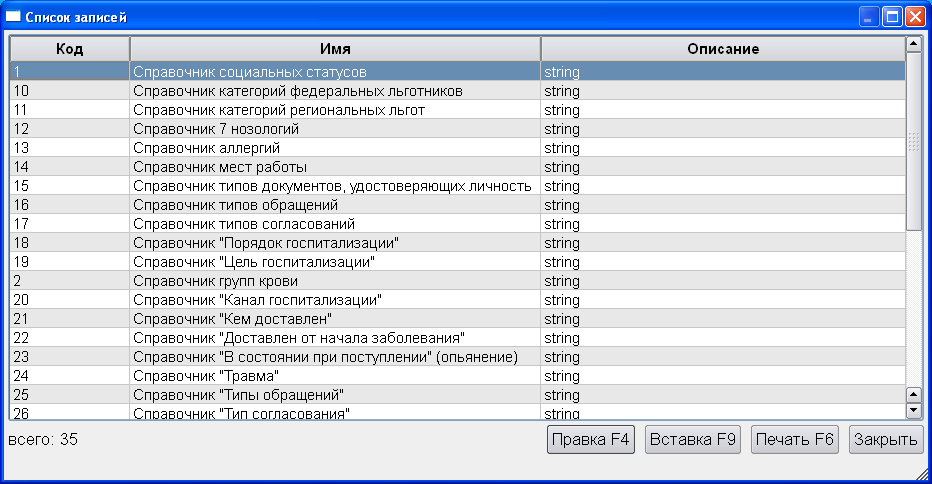
\includegraphics[width = 0.7\textwidth ,keepaspectratio]{spr_flatdir}
 \caption{Редактор плоских справочников}
 \label{img_spr_flatdir}
\end{figure} 

При создании справочника необходимо указать следующие данные:
\begin{itemize}
 \item \dm{Название} справочника;
 \item \dm{Код} -- уникальный код плоского справочника;
 \item \dm{Описание} -- краткое описание назначения справочника;
 \item Создать структуру справочника на вкладке \dm{Структура} (Рисунок \ref{img_spr_flatdir_card1}). Для этого необходимо установить курсор в первой свободной ячейке таблицы и последовательно заполнить поля:
  \begin{itemize}
   \item \dm{Имя} -- название поля таблицы (латиницей);
   \item \dm{Описание} -- краткое описание назначения поля;
   \item \dm{Тип поля} -- тип данных, которые должны храниться в поле, выбирается из справочника;
   \item \dm{Маска} -- маска для ввода данных в поле;
   \item \dm{Обязательный} -- при установке флажка в данном поле, его заполнение на вкладке \dm{Данные} становится обязательным.
  \end{itemize}
 В таблицу можно последовательно добавить любое количество строк (полей).
 \item Заполнить таблицу данными на вкладке \dm{Данные} (Рисунок \ref{img_spr_flatdir_card2}). Ввод данных осуществляется непосредственно в таблицу.
\end{itemize}

\begin{figure}[!ht]\centering
 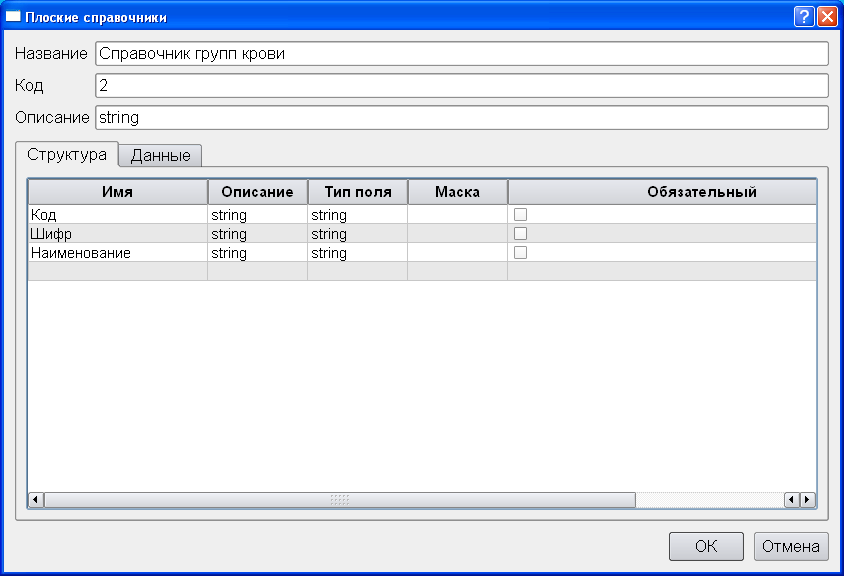
\includegraphics[width = 0.7\textwidth ,keepaspectratio]{spr_flatdir_card1}
 \caption{Редактирование структуры плоского справочника}
 \label{img_spr_flatdir_card1}
\end{figure} 

\begin{figure}[!ht]\centering
 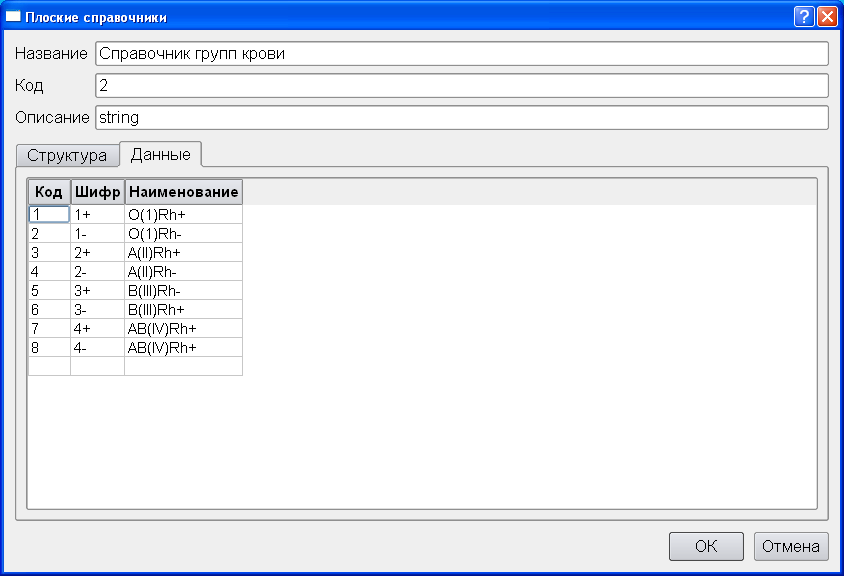
\includegraphics[width = 0.7\textwidth ,keepaspectratio]{spr_flatdir_card2}
 \caption{Редактирование данных плоского справочника}
 \label{img_spr_flatdir_card2}
\end{figure} 

После того как все данные справочника заполнены, необходимо сохранить его, нажав кнопку \btn{OK} в правом нижнем углу окна. В дальнейшем возможно добавление полей и данных в ранее созданный справочник. Удаление полей из справочника и самих справочников невозможно. 
 
\subsection{Справочник <<Организации>>}

Справочник организаций должен в обязательном порядке содержать:
\begin{itemize}
 \item 	запись о базовом ЛПУ.
\end{itemize}

Рекомендуется так же внести в справочник организаций следующие данные:
\begin{itemize}
 \item Страховые медицинские организации (СМО);
 \item Медицинские организации, с которыми может взаимодействовать базовое ЛПУ (в частности, направление пациентов и прием направленных из других ЛПУ пациентов);
 \item Организации-работодатели, заключившие договора на обслуживание в ЛПУ, а так же крупные организации, находящиеся в зоне обслуживания ЛПУ.
\end{itemize}

Справочник ЛПУ представляет собой линейную структуру (Рисунок \ref{img_spr_org}) и открывается запуском из меню \mm{Справочники \str Организации \str Организации}.
 
\begin{figure}[ht]\centering
 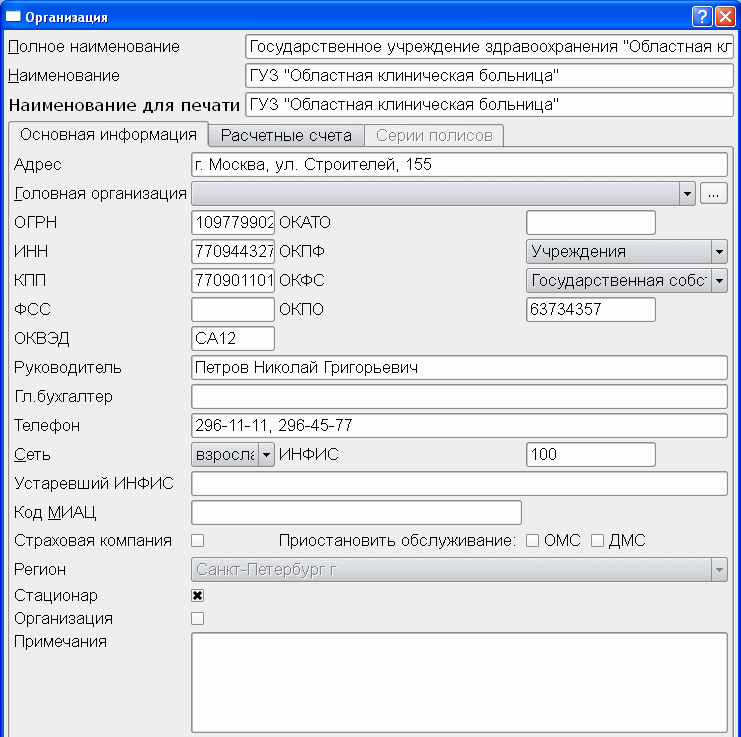
\includegraphics[width = 0.7\textwidth ,keepaspectratio]{spr_orgcard}
 \caption{Регистрационная карточка организации}
 \label{img_spr_orgcard}
\end{figure} 

При добавлении нового элемента справочника (Рисунок \ref{img_spr_orgcard}) следует обратить внимание на заполнение следующих полей:
\begin{itemize}
 \item \dm{Наименование} – наименование организации, которое будет отображаться в системе;
 \item \dm{Наименование для печати} – наименование организации, которое должно отображаться в печатных формах и отчетах;
 \item \dm{Головная организация} – данное поле заполняется, если текущая организация является филиалом. Головная организация выбирается из списка ранее зарегистрированных организаций.
 \item \dm{Сеть} – обязательно должно быть заполнено, если организация является ЛПУ.
 \item \dm{ИНФИС} – код организации. Обязательно должен быть заполнен, если организация является ЛПУ.
 \item Флажок \dm{Страховая компания} должен быть обязательно установлен, если организация является СМО. При этом требуется указать регион принадлежности СМО в поле ниже.
 \item Флажок \dm{Стационар} должен быть установлен для ЛПУ, имеющих в своем составе стационар.
 \item Флажок \dm{Организация} должен быть установлен для организаций-работодателей.
\end{itemize}

Поля \dm{Полное наименование}, \dm{Наименование}, \dm{ОГРН}, \dm{ИНН}, \dm{КПП}, \dm{ОКВЭД}, \dm{ОКПФ}, \dm{ОКФС} являются обязательными для заполнения. В них следует ввести реквизиты организации.

\begin{prim}
Название и состав полей в карточке организации может быть изменен настройками системы.
\end{prim}

На вкладке \dm{Расчетные счета} можно указать расчетные счета организации. Для корректного заполнения данных, необходимо предварительно внести банк, в котором открыт расчетный счет, в справочник \dm{Банки}. Заполнение данных о расчетных счетах выполняется непосредственно в таблице.
\begin{itemize}
 \item \dm{Расчетный счет} – 20-тизначный расчетный счет организации в банке.
 \item \dm{Банк} – выбирается из справочника банков.
 \item \dm{Наименование банка} – наименование организации, как она зарегистрирована в банке.
 \item \dm{Нал} – Вид оплаты. Флажок должен быть установлен при оплате наличными.
\end{itemize}

Для СМО на вкладке \dm{Серии полисов} можно указать серии полисов, принадлежащие данной СМО. Тогда при вводе данной серии в регистрационной карточке пациента будет автоматически подставляться название соответствующей страховой компании.

\subsection{Справочник <<Структура ЛПУ>>}

Справочник \dm{Структура ЛПУ} представляет собой древовидную структуру, содержащую информацию о подразделениях ЛПУ с учетом их иерархии (Рисунок \ref{img_spr_str}). Вызов справочника осуществляется из главного меню \mm{Справочники \str Персонал \str Структура ЛПУ}.

Регистрационная карточка подразделения содержит подробную информацию о каждом подразделении и состоит из нескольких вкладок (Рисунок \ref{img_spr_strcard}):
\begin{itemize}
 \item Вкладка \dm{Основная информация} содержит основные данные о подразделении. В большинстве случаев на начальном этапе внедрения достаточно заполнения данной вкладки.
 \item Вкладка \dm{Зона обслуживания} задает территорию обслуживания, если подразделение является участком. Доступна только при выборе значения в поле \dm{Участок} на вкладке \dm{Основная информация}. На данной вкладке необходимо зарегистрировать каждый дом, расположенный на выбранном участке.
 \item Вкладка \dm{Койки} должна содержать список коек, если подразделение является стационаром. Доступна только при установке флажка \dm{Имеет койки} на вкладке \dm{Основная информация}.
 \item Вкладка \dm{Работы} содержит список доступных в подразделении видов работ.
 \item На вкладке \dm{Перерывы} можно задать перерывы в работе для определенных сотрудников или сотрудников заданной специальности.
 \item На вкладке \dm{Типы событий} задается список типов событий, которые доступны в данном подразделении. Регистрация других типов событий в данном подразделении невозможна.
 \item На вкладке \dm{Типы действий} задается список типов действий, доступных для указанного подразделения. Они будут отображаться по умолчанию при регистрации нового действия сотрудниками указанного подразделения. Для выбора другого типа действия необходимо будет снять флажок \dm{Только разрешенные в этом отделении} окна выбора типов действий.
 \item Вкладка \dm{Запрет обслуживания} подразделением определенных категорий пациентов (по типу прикрепления).
 \item Вкладка \dm{Склад} содержит перечень доступных медикаментов. Доступна только при установке флажка \dm{Склад} на вкладке \dm{Основная информация}.
\end{itemize}
 
\begin{figure}[ht]\centering
 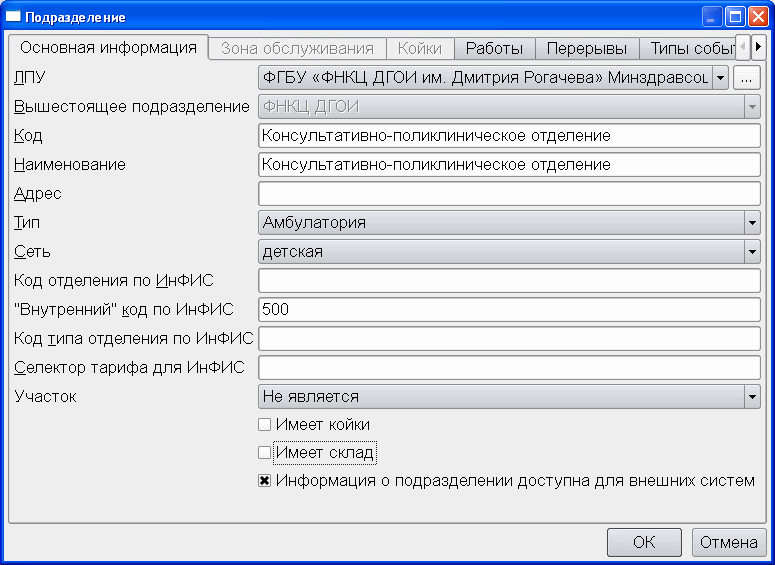
\includegraphics[width = 0.7\textwidth ,keepaspectratio]{spr_strcard}
 \caption{Регистрационная карточка подразделения}
 \label{img_spr_strcard}
\end{figure} 

Состав и описание полей всех вкладок приведено в таблице  \ref{tbl_spr_strcard}.

{\small
\begin{longtable}{|p{0.55cm}|p{4cm}|p{12cm}|}
\caption{Поля регистрационной карточки подразделения \label{tbl_spr_strcard}} \\
\hline \rule{0pt}{15pt} \centering \textbf{N пп} & \centering \textbf{Название} & \hfil \textbf{Описание поля} \\ \hline
\endfirsthead
\hline \rule{0pt}{15pt} \centering \textbf{N пп} & \centering \textbf{Название} & \hfil \textbf{Описание поля} \\ \hline
\endhead
\multicolumn{3}{|l|}{\textbf{Основная информация}} \\ \hline
1	& ЛПУ &	Базовое ЛПУ \\ \hline
2 &	Вышестоящее подразделение	& Вышестоящее подразделение по уровню иерархии в дереве. Устанавливается автоматически в соответствии с уровнем иерархии, в который добавляется элемент. Изменить вышестоящее подразделение можно перетаскиванием данного элемента в левой части справочника \dm{Структура ЛПУ} на другой уровень. \\ \hline
3	& Код &	Обозначение подразделения, которое будет отображаться в иерархическом дереве \\ \hline
4	& Наименование &	Наименование подразделения для внешних систем \\ \hline
5	& Адрес	& Заполняется только для обособленных подразделений, расположенных по адресу, отличному от адреса основного ЛПУ \\ \hline
6	& Тип &	Тип подразделения выбирается из справочника \\ \hline
7 &	Сеть & Выбирается из справочника \mm{Справочники \str Организации \str Сеть} \\ \hline
8 &	Код отделения по ИнФИС	& Внешний код подразделения в системе региона \\ \hline
9	& <<Внутренний>> код по ИнФИС &	Внутренний код подразделения \\ \hline
10 &	Код типа отделения по ИнФИС &	Код типа отделения в системе региона \\ \hline
11	& Селектор тарифа для ИнФИС & \\ \hline	
12 & Участок &	Если подразделение является участком, то необходимо выбрать тип участка из списка, после чего становится доступной вкладка \dm{Зона обслуживания} \\ \hline
13 &	Имеет койки	& Необходимо установить данный флажок, если подразделение является стационаром и имеет койки, после чего становится доступной вкладка \dm{Койки} \\ \hline
14	& Имеет склад &	Необходимо установить данный флажок, если подразделение имеет запас медикаментов, после чего становится доступной вкладка \dm{Склад} \\ \hline
15	& Информация о подразделении доступна для внешних систем & \\ \hline	
\multicolumn{3}{|l|}{\textbf{Зона обслуживания}} \\ \hline
1	& Город &	Выбирается из справочника КЛАДР \\ \hline
2	& Улица & 	Выбирается из справочника КЛАДР \\ \hline
3	& Дом & \\ \hline 	
4	& Корпус	& \\ \hline
5	& Первая кв. &	Начало интервала квартир, принадлежащих данному участку \\ \hline
6	& Последняя кв. & Окончание интервала квартир, принадлежащих данному участку \\ \hline	
\multicolumn{3}{|l|}{\textbf{Койки}} \\ \hline
1 &	Код &	Код койки \\ \hline
2	& Наименование	& Наименование койки \\ \hline
3	& Штат	& Следует установить флажок, если койка является штатной \\ \hline
4	& Тип	& Тип койки выбирается из фиксированного списка \\ \hline
5	& Профиль	& Профиль койки выбирается из справочника \mm{Справочники \str Учет \str Профили коек} \\ \hline
6	& Смены &	Количество смен в работе койки \\ \hline
7	& Режим	& Режим койки выбирается из фиксированного списка \\ \hline
8 &	Пол	& Ограничения по полу пациентов, которые могут размещаться на койке. Если не указано, то пол пациента может быть любым \\ \hline
9 &	Возраст	& Возраст пациентов, которые могут размещаться на койке. Если не указано, то возраст может быть любым \\ \hline
10	& Начало	& Дата начала работы койки \\ \hline
11	& Окончание	& Дата окончания работы койки \\ \hline
12	& Причина сворачивания	& Причина последнего сворачивания выбирается из фиксированного списка: ремонт, карантин. \\ \hline
13	& Начало сворачивания	& Дата начала последнего сворачивания \\ \hline
14	& Окончание сворачивания	& Дата окончания последнего сворачивания \\ \hline
\multicolumn{3}{|l|}{\textbf{Работы}} \\ \hline
1 &	Тип	& Тип работ выбирается из справочника \mm{Справочники \str Учет \str Типы работ} \\ \hline
2	& Начало	& Время начала выполнения работы \\ \hline
3	& Окончание	& Время окончания выполнения работы \\ \hline
4	& Количество	& Допустимое количество работ в сутки \\ \hline
\multicolumn{3}{|l|}{\textbf{Перерывы}} \\ \hline
1 &	Наследует перерывы	& При установке данного флажка перерывы наследуются из вышестоящего подразделения в дереве. При этом на текущем уровне могут быть добавлены дополнительные перерывы \\ \hline
2	& Начало	& Время начало перерыва в работе \\ \hline
3	& Окончание	& Время окончания перерыва в работе \\ \hline
4	& Специальность	& Указывается при регистрации перерыва для всех сотрудников определенной специальности \\ \hline
5	& Сотрудник	& Указывается при регистрации перерыва для определенного сотрудника \\ \hline
\multicolumn{3}{|l|}{\textbf{Типы событий}} \\ \hline
1	& Наследует типы событий	& При установке данного флажка допустимые типы событий наследуются из вышестоящего подразделения в дереве. При этом на текущем уровне могут быть добавлены дополнительные типы событий \\ \hline 
2	& Типы событий	& Допустимые типы событий в данном подразделении; выбираются из справочника \mm{Справочник \str Учет \str Типы событий} \\ \hline
\multicolumn{3}{|l|}{\textbf{Типы действий}} \\ \hline
1	& Наследует типы действий	& При установке данного флажка допустимые типы действий наследуются из вышестоящего подразделения в дереве. При этом на текущем уровне могут быть добавлены дополнительные типы действий \\ \hline
2	& Тип	& Допустимые типы действий в данном подразделении; выбираются из справочника \mm{Справочник \str Учет \str Типы действий} \\ \hline
\multicolumn{3}{|l|}{\textbf{Запрет обслуживания}} \\ \hline
1 &	Тип прикрепления	& Выбирается из справочника \\ \hline
2 &	Способ ограничения	& Уровень ограничения выбирается из списка. При мягком и строгом уровне запрета, будут выдаваться предупреждения, но возможность обслужить пациента сохраняется. При выборе способа <<Запрет>> обслуживание пациента с указанным типом прикрепления невозможно \\ \hline
\multicolumn{3}{|l|}{\textbf{Склад}} \\ \hline
1 &	ЛСиИМ	& Наименование медикамента; выбирается из справочника \mm{Справочники \str Номенклатура \str Справочник ЛС для назначений} \\ \hline
2	& Тип финансирования	& Источник финансирования медикамента; выбирается из справочника \mm{Справочники \str Финансовые \str Источники финансирования} \\ \hline
3	& Гарантийный запас	& Гарантийный запас (количество) \\ \hline
4 &	Точка заказа	& Указывается точка заказа \\ \hline
\end{longtable}
}

\subsection{Справочник <<Сотрудники>>}

Вызов справочника \dm{Сотрудники} осуществляется из главного меню выбором пункта \mm{Справочники \str Персонал \str Сотрудники}. Справочник представляет собой линейную структуру и содержит данные обо всех сотрудниках ЛПУ, участвующих в лечебно-диагностическом процессе (в том числе, внешних совместителях), а так же идентификационные данные сотрудников для входа в \tmis.

Внешне окно справочника отличается от других справочников, так как для удобства пользователя содержит параметры фильтрации непосредственно в окне справочника (Рисунок \ref{img_spr_pers}). Для применения параметра фильтрации нужно установить напротив него флажок  \putx , а затем выбрать из списка нужное значение. Применение фильтра осуществляется автоматически после изменения параметров фильтрации.

\begin{figure}[ht!]\centering
 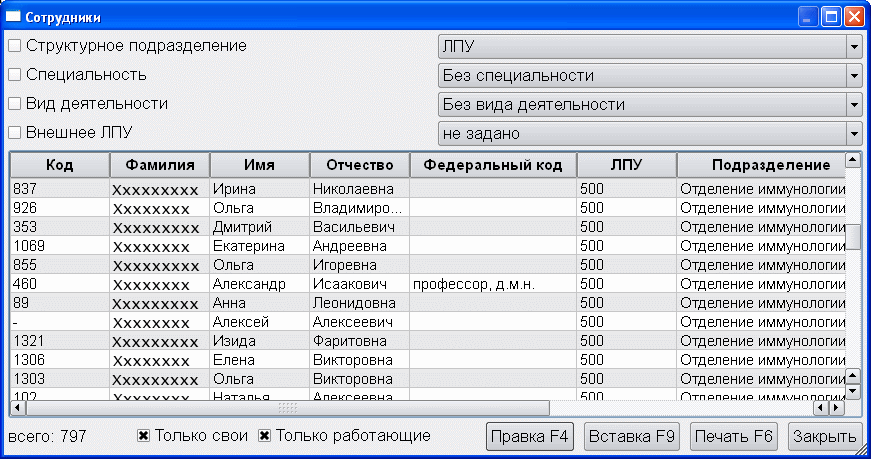
\includegraphics[width = 0.8\textwidth ,keepaspectratio]{spr_pers}
 \caption{Справочник сотрудников}
 \label{img_spr_pers}
\end{figure}

Регистрационная карточка сотрудника содержит несколько вкладок (Рисунок \ref{img_spr_strcard}):
\begin{itemize}
 \item На вкладке \dm{Общие} находится вся основная информация о сотруднике и данные пользователя \tmis.
 \item Вкладка \dm{Личные} содержит персональные данные о сотруднике.
 \item На вкладке \dm{Квалификация} можно ввести информацию о курсах повышения квалификации, пройденных сотрудником.
 \item На вкладке \dm{Кадровые перемещения} можно вести историю кадровых перемещений сотрудника.
 На вкладке \dm{Вид деятельности} могут быть указаны виды деятельности, выполняемые сотрудником.
 \item Вкладка \dm{График} содержит шаблон расписания сотрудника, а так же квоты для различных типов записи на прием. Шаблон может быть применен при формировании расписания сотрудника. Для этого следует выбрать тип заполнения <<По персональному графику>>.
\end{itemize}
 
\begin{figure}[ht!]\centering
 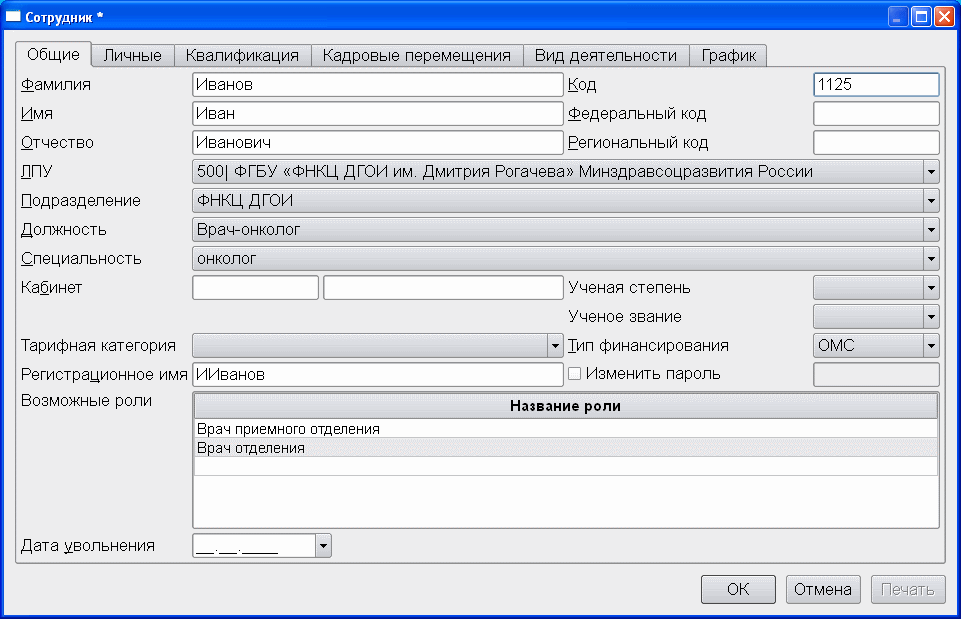
\includegraphics[width = 0.8\textwidth ,keepaspectratio]{spr_perscard}
 \caption{Карточка редактирования данных о сотруднике. Вкладка <<Общие>>}
 \label{img_spr_perscard}
\end{figure}

Описание некоторых полей регистрационной карточки сотрудника приведено в таблице \ref{tbl_spr_perscard}.

{\small
\begin{longtable}{|p{0.55cm}|p{4cm}|p{12cm}|}
\caption{Поля регистрационной карточки сотрудника (не полный перечень) \label{tbl_spr_perscard}} \\
\hline \rule{0pt}{15pt} \centering \textbf{N пп} & \centering \textbf{Название} & \hfil \textbf{Описание поля} \\ \hline
\endfirsthead
\hline \rule{0pt}{15pt} \centering \textbf{N пп} & \centering \textbf{Название} & \hfil \textbf{Описание поля} \\ \hline
\endhead
\multicolumn{3}{|l|}{\textbf{Общие}} \\ \hline
1	&  Код	& Код сотрудника в системе \\ \hline
2	& Кабинет	& Имеются 2 поля: номера основного и альтернативного (для второго приема) кабинетов, использующиеся по умолчанию при составлении расписания для сотрудника \\ \hline
3	& ЛПУ	& При указании ЛПУ, отличного от базового, сотрудник считается внешним совместителем. \\ \hline
4	& Тарифная категория	& Тарифная категория сотрудника для выставления счетов \\ \hline
5	& Тип финансирования	& Тип финансирования по умолчанию для данного сотрудника \\ \hline
6	& Регистрационное имя	& Имя пользователя, используемое сотрудником для входа в систему \\ \hline
7 &	Изменить пароль &	При установке данного флажка в следующее поле можно ввести новый пароль пользователя \\ \hline
8	& Возможные роли	& Предопределенный набор ролей пользователя в системе. При указании нескольких ролей, пользователю будет предложено выбрать одну из них в момент авторизации в системе после ввода регистрационного имени и пароля. \\ \hline
9	& Дата увольнения	& При указании данной даты, сотрудник считается уволенным с указанной даты и не отображается в списке сотрудников при установленном флажке фильтра \dm{Только работающие} \\ \hline
\multicolumn{3}{|l|}{\textbf{График}} \\ \hline
1	& (тип шаблона расписания)	& Выбирается из списка: <<Один план>> – одинаковое расписание работы на каждый день; <<Нечет\slash Чет>> - различное расписание по четным и нечетным дням месяца; <<1 неделя>> - различное расписание работы на каждый день недели; <<2 недели>> - различное расписание работы для каждого дня недели отдельно для четных и нечетных недель; <<3 недели>> - различное расписание работы на каждый день недели для каждой тройки недель; <<4 недели>> - различное расписание работы на каждый день недели для каждой четверки недель.  \\ \hline
2	& Амбулаторно	& Время амбулаторного приема \\ \hline
3	& Каб.	& Номер кабинета для амбулаторного приема \\ \hline
4	& План	& Норма приема пациентов \\ \hline
5	& Амбулаторно2 & Дополнительное время амбулаторного приема (второй прием) \\ \hline
6	& Каб.2	& Номер кабинета для дополнительного амбулаторного приема \\ \hline
7	& План2 &	Норма дополнительного приема пациентов\\ \hline
8	& Вызовы	& Время обслуживания вызовов на дом \\ \hline
9	& План	& Нормативное количество вызовов \\ \hline
10	& Вызовы2	& Дополнительное время для обслуживания вызовов на дом \\ \hline
11	& План2	& Нормативное количество дополнительных вызовов \\ \hline
12	& Информация о сотруднике доступна для внешних систем	& При установке данного флажка расписание сотрудника становится доступным при записи через внешние системы \\ \hline
13	& Расписание видимо до &	Дата, до которой данные о расписании сотрудника доступны в системе \\ \hline
14	& Расписание видимо на (дней) &	Количество дней вперед, на которое доступно расписание сотрудника, начиная от текущей даты \\ \hline
15	& Амбулаторный прием	& Норма количества пациентов, принятых за одну смену (основной и дополнительный прием) \\ \hline
16	& Вызовы на дом	& Норма количества вызовов, выполненных за смену (основное и дополнительное время) \\ \hline
16	& КЭР	& Норма количества КЭР за смену \\ \hline
17	& Первичная квота	& Доля или количество талонов, доступная для записи через регистратуру \\ \hline
18	& Врачебная квота	& Доля или количество талонов для записи сотрудником к самому себе \\ \hline
19	& Консультативная квота	& Доля или количество талонов, доступная для записи к данному сотруднику другими врачами ЛПУ \\ \hline
20	& Внешняя квота	& Доля или количество талонов, доступная для записи через внешние системы. Опция доступна только при установке флажка \dm{Информация о сотруднике доступна для внешних систем} \\ \hline
21	& Единица квотирования	& В зависимости от выбранного значения в данном поле, значения в полях 17 – 20 указываются в процентах либо в абсолютных величинах (количество) \\ \hline
\end{longtable}
}

\subsection{Справочник <<Типы событий>>}

Справочник представляет собой линейную структуру и вызывается из главного меню \mm{Справочники \str Учет \str Типы событий} (Рисунок \ref{img_spr_tpev}).

\begin{figure}[ht]\centering
 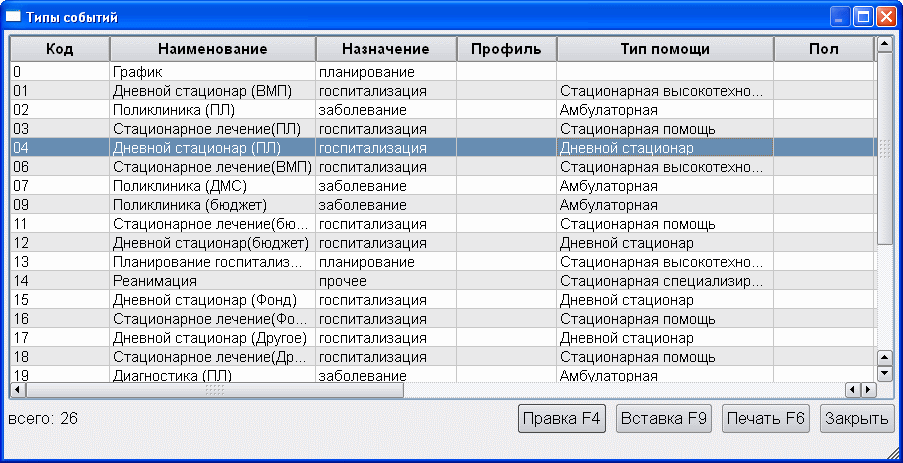
\includegraphics[width = 0.8\textwidth ,keepaspectratio]{spr_tpev}
 \caption{Справочник типов событий}
 \label{img_spr_tpev}
\end{figure}

В регистрационной карточке типа события содержится большое число настроек, размещенных на нескольких вкладках (Рисунок \ref{img_spr_tpev_card}):
\begin{itemize}
 \item Вкладка \dm{Основная информация} содержит основные настройки типа события.
 \item Вкладка \dm{Визиты} содержит настройки посещений для поликлинических и диагностических обращений.
 \item Вкладка \dm{Осмотры} включает список посещений.
 \item На вкладках \dm{Статус}, \dm{Диагностика}, \dm{Лечение} и \dm{Прочие мероприятия} содержится список медицинских документов, лабораторных и диагностических исследований, видов лечения и других мероприятий соответственно, отображаемых в окне планировщика при регистрации нового события.
\end{itemize} 

\begin{figure}[ht]\centering
 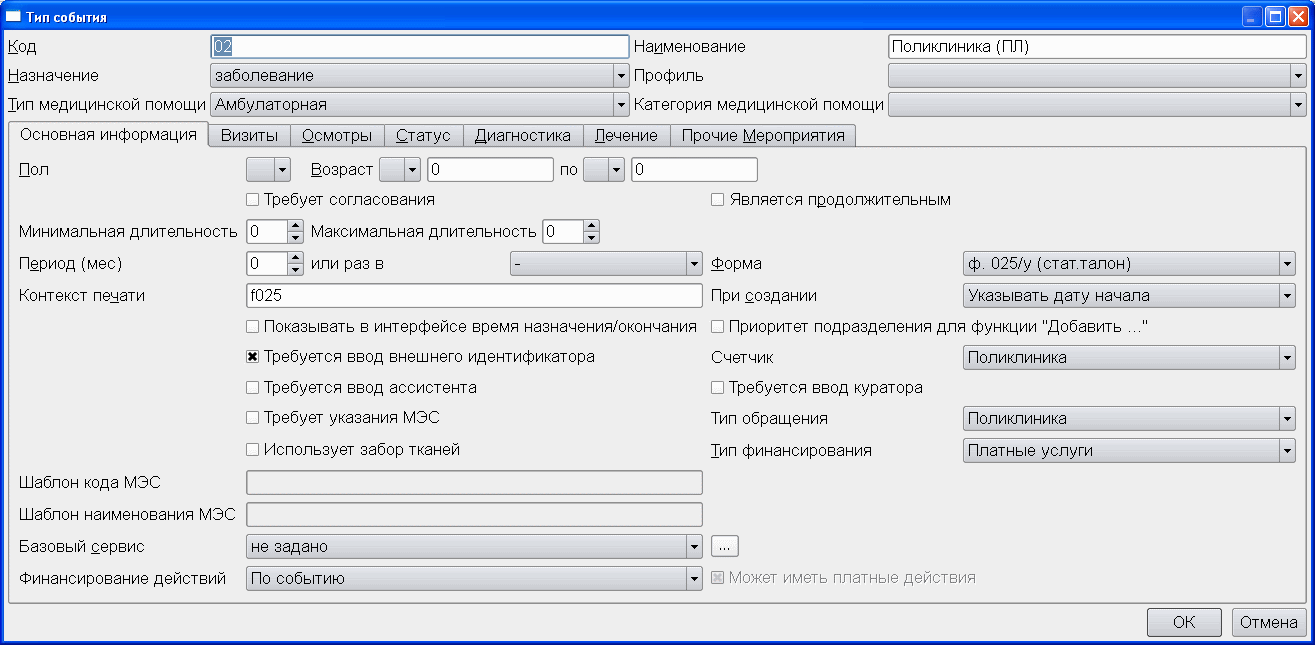
\includegraphics[width = 0.8\textwidth ,keepaspectratio]{spr_tpev_card}
 \caption{Регистрационная карточка типа события}
 \label{img_spr_tpev_card}
\end{figure}

Описание полей карточки редактирования типа события приведено в таблице \ref{tbl_spr_tpev}.

{\small
\begin{longtable}{|p{0.55cm}|p{4cm}|p{12cm}|}
\caption{Поля карточки редактирования типа события \label{tbl_spr_tpev}} \\
\hline \rule{0pt}{15pt} \centering \textbf{N пп} & \centering \textbf{Название} & \hfil \textbf{Описание поля} \\ \hline
\endfirsthead
\hline \rule{0pt}{15pt} \centering \textbf{N пп} & \centering \textbf{Название} & \hfil \textbf{Описание поля} \\ \hline
\endhead
1 &	Код	& Код типа события \\ \hline
2 &	Наименование	& Наименование события \\ \hline
3 &	Назначение	& Выбирается из справочника \mm{Справочники \str Учет \str Назначение типа события}. В зависимости от выбранного значения будет изменяться состав списка результатов события. \\ \hline
4	& Профиль	& Выбирается из справочника \mm{Справочники \str Учет \str Профили медицинской помощи} \\ \hline
5	& Тип медицинской помощи	& Выбирается из справочника \mm{Справочники \str Учет \str Типы медицинской помощи} \\ \hline
6	& Категория медицинской помощи	& Выбирается из справочника \mm{Справочники \str Учет \str Категории медицинской помощи} \\ \hline
\multicolumn{3}{|l|}{\textbf{Основная информация}} \\ \hline
1	& Пол	& Событие может быть зарегистрировано только для пациентов выбранного пола. В случае несоответствия пола пациента, событие отсутствует в списке доступных для регистрации \\ \hline
2	& Возраст (с)	& Событие может быть зарегистрировано только для пациентов, начиная с указанного возраста. Из списка следует выбрать единицу измерения возраста (<<Д>> - дни, <<Н>> - недели, <<М>> - месяцы, <<Г>> - годы), а в следующем поле указать начальный возраст в выбранной единице измерения \\ \hline
3 &	по	& Событие может быть зарегистрировано только для пациентов не старше указанного возраста. Из списка следует выбрать единицу измерения возраста (см. п.2), а в поле указать конечный возраст в выбранной единице измерения \\ \hline
4	& Является продолжительным	& Признак продолжительности события \\ \hline
5	& При создании	& Определяет, указывать ли при регистрации события дату начала и дату завершения события (настройка внешнего вида окна регистрации события) \\ \hline
6	& Использует забор тканей	& Не используется \\ \hline
7	& Показывать в интерфейсе время назначения/окончания	& Определяет, показывать ли при регистрации события окно ввода времени начала и окончания события (настройка внешнего вида окна регистрации события) \\ \hline
8	& Приоритет подразделения для функции <<Добавить…>>	& Не используется \\ \hline
9	& Требуется ввод внешнего идентификатора	& При установке данного флажка становится доступным поле \dm{Счетчик} \\ \hline
10	& Минимальная длительность	& Минимальная длительность события в днях \\ \hline
11	& Максимальная длительность	& Максимальная длительность события в днях \\ \hline
12	& Период (мес.)	& Периодичность события в месяцах \\ \hline
13	& или раз в &	Периодичность события (если не указана в п.12) 1 раз в выбранный период (неделю, месяц, квартал …) \\ \hline
14	& Счетчик	& Выбор типа счетчика для присвоения номера событию. Для использования поля необходимо установить флажок \dm{Требуется ввод внешнего идентификатора} \\ \hline
15	& Тип обращения	& Выбирается из справочника \mm{Справочники \str Учет \str Типы обращений} \\ \hline
16	& Тип финансирования	& Выбирается из справочника \mm{Справочники \str Финансовые \str Источники финансирования} \\ \hline
17	& Контекст печати	& Наименование контекста печати для привязки шаблонов печатных форм к типу события \\ \hline
18	& Требует согласования	& Не используется \\ \hline
19	& Требуется ввод ассистента	& Не используется \\ \hline
20	& Требуется ввод куратора	& Не используется \\ \hline
21	& Требует указания МЭС	& При установке данного флажка становятся активными поля \dm{Шаблон кода МЭС} и \dm{Шаблон наименования МЭС} \\ \hline
22	& Шаблон кода МЭС	& Часть кода медико-экономического стандарта. При регистрации события осуществляется подбор кода МЭС и привязка его к событию \\ \hline 
23	& Шаблон наименования МЭС	& Часть наименования медико-экономического стандарта. При регистрации события осуществляется подбор наименования МЭС по шаблону и привязка его к событию \\ \hline
24	& Базовый сервис	& Услуга по умолчанию для визитов, регистрируемых в событии. Выбирается из справочника \mm{Справочники \str Финансовые \str Услуга (профиль ЕИС)}. При нажатии кнопки \btn{\rule{0pt}{5pt}...}  открывается окно фильтрации услуг \\ \hline
25	& Финансирование действий	& Способ финансирования действий, входящих в состав события выбирается из списка \\ \hline
26 &	Может иметь платные действия	& Флажок доступен при выборе в поле \dm{Тип финансирования} любого значения, кроме платных услуг и устанавливается, если в состав события по выбранному типу финансирования могут включаться платные услуги \\ \hline
\multicolumn{3}{|l|}{\textbf{Визиты}} \\ \hline
1 &	Модификатор сервиса визита	& Правила модификации услуг для посещений, регистрируемых в составе события \\ \hline
2	& Место визита	& Место визита, указываемое по умолчанию для посещений. Выбирается из справочника \mm{Справочники \str Учет \str Место выполнения визитов} \\ \hline
3	& Финансирование визита	& Способ финансирования посещений по умолчанию \\ \hline
4	& Фильтрация списка услуг визитов & \\ \hline	
\multicolumn{3}{|l|}{\textbf{Осмотры}} \\ \hline
1	& Специальность	& Не используется \\ \hline 
2	& Пол	& Не используется  \\ \hline
3	& Возраст	& Не используется  \\ \hline
4	& Код МКБ по умолчанию	& Не используется  \\ \hline
5	& ДН по умолчанию	& Не используется \\ \hline
6	& ГЗ по умолчанию	& Не используется \\ \hline
7	& Тип визита	& Не используется \\ \hline
8	& Действителен	& Не используется \\ \hline
9	& Группа выбора	& Не используется \\ \hline
\multicolumn{3}{|l|}{\textbf{Статус, Диагностика, Лечение, Прочие мероприятия}} \\ \hline
1	& Наименование	& Наименование действия, выбирается из справочника \mm{Справочники \str Учет \str Типы действий} \\ \hline
2	& Специальность	& Специальность врача \\ \hline
3	& Ученая степень &	Ученая степень врача \\ \hline
4	& Тип ткани & \\ \hline	
5	& Пол	& Действие отображается в планировщике только для пациентов указанного пола \\ \hline
6	& Возраст	& Действие отображается в планировщике только для пациентов указанного возраста \\ \hline
7	& Действителен	& Период в месяцах, в течении которого действительно выполнение данного действия \\ \hline
8	& Группа выбора &	1 – обязателен для выбора, 0 – необязателен для выбора, но отображается в планировщике, [2;$\infty$ ] – нужно обязательно выбрать одно значение из группы, [-$\infty$ ;-1] – можно выбрать одно значение из группы \\ \hline
8	& Выставлять	& При установке данного флажка, действие включается в счет \\ \hline
9	& Платно	& При выборе значения <<По событию>> - возможность выполнения действия платно берется из события, <<по выбору>> - возможность выполнения действия на платной основе выбирается пользователем, <<обязательно>> - указанное действие может выполняться только платно \\ \hline
10	& Показывать в планировщике необязательные мероприятия & \\ \hline	
11	& Ограничить ввод мероприятий указанным списком &	В событие невозможно добавить действия, отсутствующие в списке \\ \hline
\end{longtable}
}
 
\subsection{Справочник <<Типы действий>>}

Справочник типов действий имеет иерархическую структуру (Рисунок \ref{img_spr_tpact}) и может быть вызван из главного меню \mm{Справочники \str Учет \str Типы действий}.

\begin{figure}[ht]\centering
 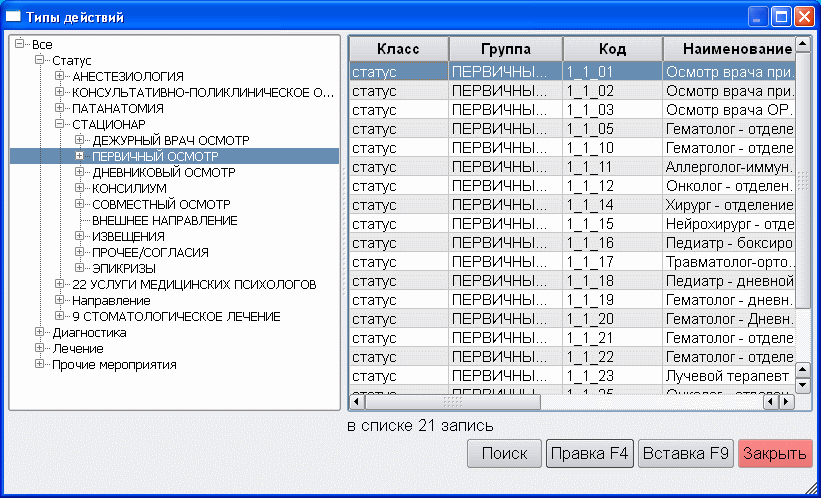
\includegraphics[width = 0.7\textwidth ,keepaspectratio]{spr_tpact}
 \caption{Справочник типов действий}
 \label{img_spr_tpact}
\end{figure}

Справочник содержит описание всех типов действий, использующихся в системе. Информация размещается на нескольких вкладках:
\begin{itemize}
 \item Вкладка \dm{Основная информация} содержит общие настройки типа действия, настройки доступности действия и интерфейсные настройки.
 \item На вкладке \dm{Умолчания} можно настроить значения, которые будут подставляться при создании типа действий по умолчанию.
 \item На вкладке \dm{Свойства} располагается список свойств действия и их настройки.
 \item На вкладке \dm{Оплата\slash Квотирование} осуществляется связь типов действий с услугами, а так же связь типов действий и видов квот.
 \item На вкладке \dm{Забор тканей} вводится список биоматериалов, необходимых для исследования, описываемого данным типом действия. Заполнение данных на вкладке требуется при интеграции с ЛИС <<Алтей>>.
 \item Вкладка \dm{Проверка} позволяет ввести критерии контроля действий в составе события при закрытии обращения.
\end{itemize}

\begin{figure}[ht!]\centering
 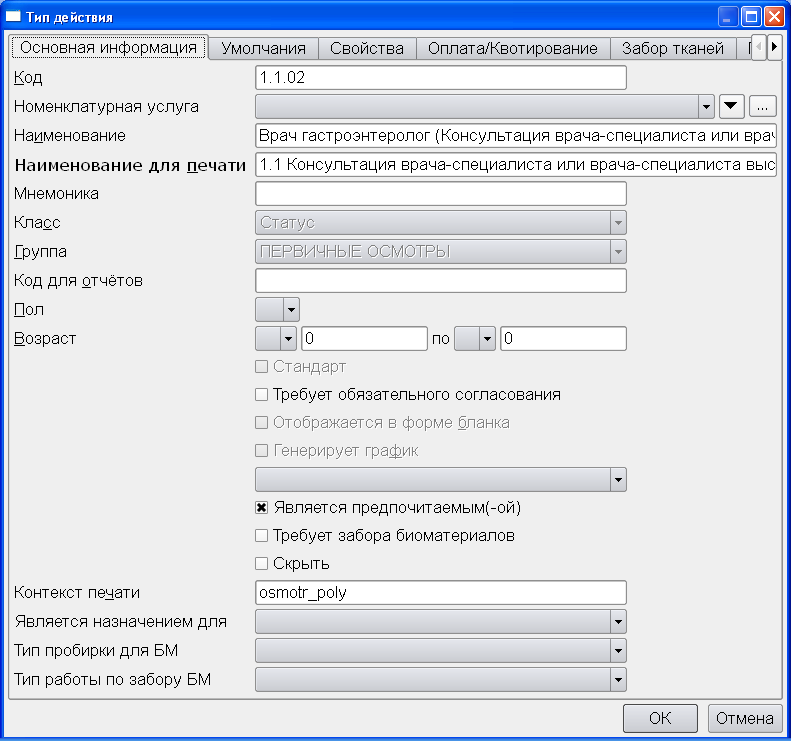
\includegraphics[width = 0.7\textwidth ,keepaspectratio]{spr_tpact_card}
 \caption{Карточка редактирования типа действия}
 \label{img_spr_tpact_card}
\end{figure}

Подробное описание полей карточки редактирования типа действия приведено в таблице \ref{tbl_spr_tpact}.

{\small
\begin{longtable}{|p{0.55cm}|p{4cm}|p{12cm}|}
\caption{Поля карточки редактирования типа действий \label{tbl_spr_tpact}} \\
\hline \rule{0pt}{15pt} \centering \textbf{N пп} & \centering \textbf{Название} & \hfil \textbf{Описание поля} \\ \hline
\endfirsthead
\hline \rule{0pt}{15pt} \centering \textbf{N пп} & \centering \textbf{Название} & \hfil \textbf{Описание поля} \\ \hline
\endhead
\multicolumn{3}{|l|}{\textbf{Основная информация}} \\ \hline
1 &	Код	& Код типа действия. Для типов действий, описанных в таблице 15, значение кода должно строго соответствовать кодам, указанным в таблице в поле \dm{Код} \\ \hline
2 & Номенклатурная услуга & Код услуги по классификации Минздрава РФ, соответствующей данному типу действия \\ \hline
3 &	Наименование	& Наименование типа действия, как оно будет отображаться в справочнике \\ \hline
4 &	Наименование для печати	& Наименование типа действия для использования в печатных формах \\ \hline
5 & Мнемоника & Мнемоника для типа действия \\ \hline
6	& Класс	& Устанавливается автоматически в соответствии с расположением типа действия в иерархическом дереве справочника. Для изменения значения данных полей, нужно перетащить его в иерархическом справочнике на нужный уровень, используя левую кнопку мыши. Выбранный класс определяет, в каком разделе карточки обращения будут регистрироваться действия данного типа: <<Статус>> - в разделе \dm{Медицинские документы}, <<Диагностика>> - в разделе \dm{Лабораторные и диагностические исследования}, <<Лечение>> - в разделе \dm{Лечение}, <<Прочие мероприятия>> - в разделе \dm{Движение пациента} и определяет некоторые особенности карточки типа действия  \\ \hline
7 &	Группа & Родительский элемент для данного типа действий в дереве структуры типов действий \\ \hline	
8 &	Код для отчетов	& Мнемоника, использующаяся для идентификации особых типов действий. Список доступных значений данного поля приведен в таблице 15 в поле \dm{Мнемоника}  \\ \hline
9	& Пол	& При указании пола, добавление действия становится возможным только в события пациентов выбранного пола  \\ \hline
10	& Возраст	& Состоит из 4-х контролов: 2 из них задают начало интервала возрастов, а оставшиеся 2 – окончание интервала. В каждой группе в первом элементе из списка выбирается единица измерения возраста (<<Д>> - дни, <<Н>> - недели, <<М>> - месяцы, <<Г>> - годы), а во втором – указывается значение возраста. При указании интервала возрастов, добавление действия данного типа становится возможным только для пациентов, возраст которых попадает в заданный интервал  \\ \hline
11	& Стандарт	& Не используется  \\ \hline
12	& Требует обязательного согласования &  Для платных услуг \\ \hline
13	& Отображается в форме бланка	& Не используется \\ \hline 
14	& Генерирует график	& Не используется \\ \hline
15	& Является предпочитаемым(-ой) &  \\ \hline
16	& Требует забора биоматериалов	& Не работает. Добавление поля \dm{Тип биоматериала} в карточку редактирования действия осуществляется для всех действий класса <<Диагностика>> \\ \hline
17 & Скрыть & Скрыть тип действия для пользователя \\ \hline
18	& Контекст печати	& Наименование контекста печати для привязки шаблонов печатных форм к типу действия  \\ \hline	
19	& Является назначением для	&  \\ \hline
20	& Тип пробирки для БМ	& Тип пробирки выбирается из справочника \mm{Справочники \str Лаборатория \str Типы пробирок} \\ \hline
21	& Тип работы по забору БМ	& Выбирается из справочника \mm{Справочники \str Учет \str Типы работ} \\ \hline
\multicolumn{3}{|l|}{\textbf{Умолчания}} \\ \hline
1	& Показывать в интерфейсе время назначения\slash начала\slash окон\-ча\-ния &	При установке данного флажка в шапке карточки редактирования действия данного типа отображаются поля для ввода даты и времени назначения, начала и окончания действия. При снятии данного флажка будут отображаться только поля для ввода даты назначения, начала и окончания действия (без уточнения времени)  \\ \hline
2	& Состояние	& Состояние, в котором будет находиться действие при создании  \\ \hline
3	& Планируемая дата выполнения &	Правило установки значения поля \dm{План} по умолчанию в карточке редактирования действия \\ \hline
4	& Дата окончания	& Правило установки значения поля \dm{Выполнено} по умолчанию в карточке редактирования действия \\ \hline
5	& Дата назначения	& Правило установки значения поля \dm{Назначено} по умолчанию в карточке редактирования действия \\ \hline
6	& Исполнитель по умолчанию &	Можно выбрать фамилию сотрудника, который будет устанавливаться в качестве исполнителя при создании действия \\ \hline
7	& Исполнитель в событии &	Правило заполнения поля \dm{Исполнитель} значением по умолчанию при первом открытии на редактирование действия из карточки обращения \\ \hline
8	& Исполнитель в отд.редакторе	& Правило заполнения поля \dm{Исполнитель} значением по умолчанию при первом открытии на редактирование действия ВНЕ карточки обращения, например из вкладки \dm{Обслуживание} \\ \hline
9	& Количество	& Состоит из двух контролов: в первом поле можно ввести значения количества, которое будет установлено по умолчанию, во втором – из списка выбирается правило задания количества. При выборе значения из списка <<Количество вводится непосредственно>> в действии указывается количество, введенное в первое поле, но пользователь может изменить его; при выборе значения <<Ограничить заданным количеством>> в карточке редактирования действия в поле \dm{Количество} указывается заданное значение, которое недоступно для редактирования пользователю; при выборе другого варианта из списка – количество в карточке редактирования действия вычисляется автоматически \\ \hline
10	& Максимальное количество в событии &	Максимально допустимое количество действий данного типа, которые могут быть добавлены в одно событие (при указании значения <<0>> количество действий не ограничено)  \\ \hline
11	& Кабинет	& Номер кабинета по умолчанию для действий данного типа \\ \hline
\multicolumn{3}{|l|}{\textbf{Свойства}} \\ \hline
1 &	Шаблон	& Наименование свойства выбирается из справочника \mm{Справочники \str Учет \str Библиотека свойств действий}. При выборе шаблона, наименование и описание свойства подставляются автоматически из библиотеки \\ \hline
2 &	Наименование	& Наименование свойства, которое будет отображаться в карточке редактирования действия \\ \hline
3	& Описание	& Описание свойства (Для администратора) \\ \hline
4	& Ед.Изм. &	Единица измерения для величины, описанной в свойстве \\ \hline
5	& Тип	& Описание типов свойств приведено в таблице 7 \\ \hline
6	& Область & В данном поле указывается значение в зависимости от выбранного типа (см. п. 5). Для некоторых типов заполнение не требуется. Параметры заполнения данного поля приведены в таблице 7 \\ \hline
7	& Штраф	& Штраф за незаполнение свойства (в баллах) \\ \hline
8	& Значение по умолчанию	& Значение свойства, устанавливаемое по умолчанию \\ \hline
9	& Вектор	& Не используется \\ \hline
10	& Норматив	& Границы нормы в выбранной единице измерения (как правило, используется для лабораторных исследований). Начало и конец границ задаются через тире, например <<2,6-8>> задает границы нормы от 2.6 до 8.  \\ \hline
11	& Пол	& При указании пола пациента, данное свойство отображается только для пациентов выбранного пола \\ \hline
12	& Возраст	& При указании интервала возраста, данное свойство отображается только для пациентов, возраст которых попадает в заданный интервал. Интервал вводится через тире с указанием единицы измерения, например <<1Г-10Г>> = от 1 до 10 лет, <<-6М>> = от 0 до 6 месяцев \\ \hline
13	& Видимость при выполнении работ	& При установке флажка, данное свойство отображается в окне редактирования работ \\ \hline
14	& Назначаемый	& При установке этого флажка, для данного свойства появляется флажок в столбце \dm{Назначено} карточки редактирования действий (для лабораторных исследований)  \\ \hline
15	& В эпикриз	& При установке флажка, значение данного свойства становится доступно для включения в эпикриз \\ \hline
16	& Тест	& Выбирается из справочника \mm{Справочники \str Лаборатория \str Показатели исследований} (для связи с ЛИС) \\ \hline
17	& Оценка	& Тип оценки результата исследования (для лабораторных исследований) \\ \hline
18	& Код	& Код группировки и идентификации свойств действий. Подробное описание данного поля приведено в п. \ref{spr_kod}  \\ \hline
19	& Обязательное	& При установке данного флажка, поле обязательно для заполнения \\ \hline
20	& Только для чтения	& При установке данного флажка, редактирование поля невозможно \\ \hline
\multicolumn{3}{|l|}{\textbf{Оплата/Квотирование}} \\ \hline 
1 &	Услуга по умолчанию	& Услуга, связываемая с действием при отсутствии подходящего варианта в таблице \dm{Услуга в зависимости от типа финансирования} \\ \hline
2	& Тип финансирования	& Выбирается из справочника \mm{Справочники \str Финансовые \str Источники финансирования} \\ \hline
3	& Услуга	& Услуга, связываемая с действием, если источник финансирования события совпадает с источником финансирования, указанным в данной строке. Выбирается из справочника \mm{Справочники \str Финансовые \str Услуга (профиль ЕИС)} \\ \hline
4	& Вид квоты по умолчанию	& Вид квоты, связываемый с данным действием по умолчанию, при отсутствии подходящего варианта в таблице \dm{Квотирование}. Выбирается из справочника \mm{Справочники \str Учет \str Виды квот}  \\ \hline
5	& Тип финансирования	& Выбирается из справочника \mm{Справочники \str Финансовые \str Источники финансирования} \\ \hline
6	& Класс квоты	& Выбирается из справочника \mm{Справочники \str Учет \str Виды квот} \\ \hline
7	& Вид квоты	& Вид квоты, связываемый с действием, если источник финансирования события совпадает с источником финансирования, указанным в данной строке. Выбирается из справочника \mm{Справочники \str Учет \str Виды квот} \\ \hline
\multicolumn{3}{|l|}{\textbf{Забор тканей}} \\ \hline
1	& Тип ткани	& Выбирается из справочника \mm{Справочники \str  Лаборатория \str Типы тканей} \\ \hline
2	& Количество	& Указывается количество биоматериала (целое число) \\ \hline
3	& Ед.измерения	& Единица измерения количества биоматериала \\ \hline
\multicolumn{3}{|l|}{\textbf{Проверки}} \\ \hline 
1 &	Тип события	& Выбирается из справочника \mm{Справочники \str Учет \str Типы событий}. Если необходимо указать обязательность наличия данного действия в каком-либо событии, следует указать этот тип события в данном поле, а остальные поля оставить пустыми \\ \hline
2	& Связанный тип действия &	Выбирается из справочника \mm{Справочники \str Учет \str Типы действий}. Выбирается действие, соотношение с которым необходимо задать для текущего действия. \\ \hline
3	& Тип соответствия	& Тип соответствия для текущего действия и действия, выбранного в поле \dm{Связанный тип действия} в событии, указанном в поле \dm{Тип события}. При выборе значения <<И>> (по умолчанию) – необходимо, чтобы в событии присутствовали оба действия; <<ИЛИ>> - в событии должно присутствовать одно из действий; <<НЕ>> - при наличии в событии текущего действия, действие связанного типа присутствовать не может \\ \hline
\end{longtable}
}

В таблице \ref{tbl_spr_tpact_prop} приведено описание типов свойств действий.

{\small
\begin{longtable}{|p{0.55cm}|p{3.5cm}|p{6.1cm}|p{6.1cm}|}
\caption{Типы свойств действий \label{tbl_spr_tpact_prop}} \\
\hline \rule{0pt}{15pt} \centering \textbf{N пп} & \centering \textbf{Название типа} & \centering \textbf{Описание типа} & \hfil \textbf{Область} \\ \hline
\endfirsthead
\hline \rule{0pt}{15pt} \centering \textbf{N пп} & \centering \textbf{Название типа} & \centering \textbf{Описание типа} & \hfil \textbf{Область} \\ \hline
\endhead
1 &	Double	& Вещественное число	& ---  \\ \hline
2 &	Integer	& Целое число	& --- \\ \hline
3 &	String	& Строка	& В одинарных кавычках через запятую можно указать возможные значения для того, чтобы пользователь выбирал из предложенного списка. Если последним элементом списка указать символ <<*>> без кавычек, то пользователь сможет ввести свое значение (не из списка). Если символ <<*>> в конце не указан, то доступные варианты значений поля будут ограничены указанным списком \\ \hline
4 &	Date &	Дата	& --- \\ \hline
5	& Time &	Время &	--- \\ \hline
6	& Reference	& Ссылка на справочник системы	& Название таблицы БД справочника \\ \hline
7	& Text	& Текст	& --- \\ \hline
8	& Html	& Результат выполнения шаблона печати &	Контекст шаблона печати \\ \hline
9	& Constructor &	Текст с возможностью выбора ключевых фраз из определенной ветки тезауруса	& Значения поля \dm{Код} соответствующего корневого узла ветки тезауруса \\ \hline
10	& Жалобы &	Текст с возможностью выбора ключевых фраз из справочника \mm{Справочники \str Медицинские \str Жалобы} & --- \\ \hline
11	& RLS &	Ссылка на запись схемы данных rls &	--- \\ \hline
12	& Organisation & Ссылка на запись справочника \mm{Справочники \str Организации \str Организации} &	Можно указать тип организации, например <<ЛПУ>> \\ \hline
13	& OrgStructure &	Ссылка на запись справочника \mm{Справочники \str Персонал \str Структура ЛПУ} &	--- \\ \hline
14	& HospitalBed	& Ссылка на запись таблицы orgstructure\_hospitalbed (Список коек, указанный в справочнике \dm{Структура ЛПУ} на вкладке \dm{Койки}) &	--- \\ \hline
15	& Person	& Ссылка на запись справочника \mm{Справочники \str Персонал \str Сотрудники} & --- \\ \hline
16	& Image &	Изображение &	--- \\ \hline
17	& HospitalBedProfile	& Ссылка на запись из справочника \mm{Справочники \str Учет \str Профили коек} &	--- \\ \hline
18 &	JobTicket &	Талон на выполнение работы	& Код вида работы \\ \hline
19	& Запись в др.ЛПУ &	Активизация функции записи в другое ЛПУ	& --- \\ \hline
20	& ImageMap	& Маркеры, нанесенные на изображение	Файл с изображением &  \\ \hline
21	& OperationType	& Ссылка на запись справочника \mm{Справочники \str Медицинские \str Типы операций} & 	--- \\ \hline
22	& MKB & Ссылка на запись справочника \mm{Справочники \str Медицинские \str Коды МКБ Х}	& --- \\ \hline
23	& AnalysisStatus & Статус анализа &	--- \\ \hline
25	& Table	& Таблица данных. Подробное описание приведено в п. \ref{spr_tp_tbl} &  Код табличного свойства типов действий  \\ \hline
\end{longtable}
}

\subsubsection{Табличный тип данных} \label{spr_tp_tbl}

Для использования табличного типа свойств действий, его следует внести в справочник \mm{Справочники \str Учет \str Табличные свойства типов действий}, заполнив следующие поля:
\begin{itemize}
 \item \dm{Наименование таблицы} – наименование табличного представления, понятное для администратора.
 \item \dm{Код} должен быть уникальным в справочнике. Его значение указывается в поле \dm{Область} свойства действия при использовании табличного типа данных.
 \item \dm{Таблица БД} – наименование таблицы БД, из которой будет производиться выборка строк для целевой таблицы.
 \item \dm{Имя поля для выборки} – наименование поля таблицы БД, по значению которого будут отбираться строки в целевую таблицу.
 \item \dm{Список отображаемых полей} – список полей целевой таблицы. Для добавления поля в список следует указать:
 \begin{itemize}
  \item \dm{Наименование} – наименование столбца целевой таблицы, которое будет видно пользователю.
  \item \dm{Столбец} – название столбца таблицы БД, из которого будет осуществляться выборка данных для указанного столбца.
  \item \dm{Связанная таблица} – название таблицы БД, являющейся справочником для указанного поля (не обязательно).
 \end{itemize}
\end{itemize}
  
Автоматически создаются следующие представления:
\begin{itemize}
 \item \dm{TRFU\_FV} – Финальные объёмы (для ТРФУ);
 \item \dm{TRFU\_LM} – Лабораторные измерения (для ТРФУ);
 \item \dm{TRFU\_OIR} – Ответ ТРФУ на запрос компонентов крови.
\end{itemize}

\subsubsection{Поле <<Код>> описания свойств действий} \label{spr_kod}

Для идентификации некоторых свойств типов действий и передачи значений в другие разделы, необходимо указание заданной мнемоники в поле \dm{Код} свойств типов действий. Значение поля \dm{Код} должно быть уникально для свойств одного типа действий. Возможные варианты значений данного поля приведены в таблице \ref{tbl_spr_kod}.

{\small
\begin{longtable}{|p{4.1cm}|p{7.6cm}|p{5cm}|}
\caption{Мнемоники поля \dm{Код} \label{tbl_spr_kod}} \\
\hline \rule{0pt}{15pt} \centering \textbf{Мнемоника} & \centering \textbf{Наименование} & \hfil \textbf{Примечание} \\ \hline
\endfirsthead
\hline \rule{0pt}{15pt} \centering \textbf{Мнемоника} & \centering \textbf{Наименование} & \hfil \textbf{Примечание} \\ \hline
\endhead
\multicolumn{3}{|l|}{\textbf{Поступление}} \\ \hline
diagReceived	& Диагноз направившего учреждения &  \\ \hline	
diagReceivedMKB	& Код МКБ-10 диагноза направившего учреждения	&  \\ \hline
orgStructStay	& Отделение поступления &  \\ \hline	
orgStructDirectedFrom & 	Направлен из &  \\ \hline	
orgStructDirection	& Направлен в отделение &  \\ \hline	
\multicolumn{3}{|l|}{\textbf{Движение}}  \\ \hline
hospitalBed &	Койка &  \\ \hline 	
timeArrival	& Время поступления &  \\ \hline	
timeLeaved	& Время выбытия &  \\ \hline	
patronage	& Патронаж &  \\ \hline	
OrgStructStay	& Отделение пребывания &  \\ \hline	
orgStructTransfer	& Переведен в отделение &  \\ \hline	
orgStructReceived	& Переведен из отделения &  \\ \hline	
\multicolumn{3}{|l|}{\textbf{Выписка}}  \\ \hline 
hospOutcome	& Исход госпитализации &  \\ \hline	
hospLength	& Продолжительность госпитализации &  \\ \hline	
resort	& Рекомендовано санаторно-курортное лечение (указывается название санатория) &  \\ \hline	
nextHospDate	& Планируемая дата следующей госпитализации (в текущем году) &  \\ \hline	
hospOrgStruct	& Отделение госпитализации &  \\ \hline	
nextHospFinance	& Источник финансирования следующей госпитализации	&  \\ \hline
\multicolumn{3}{|l|}{\textbf{Медикаментозные назначения: Терапия, Инфузионная терапия, Химио-}}  \\
\multicolumn{3}{|l|}{\textbf{терапия, Анальгезия}} \\ \hline	
voa	& Скорость введения &  \\ \hline		
moa	& Способ введения	&  \\ \hline	
nomen	& Наименование &  \\ \hline		
units	& Единицы измерения дозировки	&  \\ \hline	
dosage	& Дозировка	&  \\ \hline	
nomen\_\%i, units\_\%i, dosage\_\%i	& &	\%i - номер группы, используется в Инфузионной терапии, в частности  \\ \hline	
\multicolumn{3}{|l|}{\textbf{Вывод данных в <<Мониторинг состояния>> web-клиента}}  \\ \hline
PULS &	ЧСС &  \\ \hline	
BPRAD	& АД диастолическое (нижнее) &  \\ \hline	
BPRAS	& АД систолическое (верхнее) &  \\ \hline	
TEMPERATURE	& Температура тела &  \\ \hline	
GROWTH 	& Рост  &  \\ \hline	
WEIGHT	& Вес	&  \\ \hline
STATE	& Состояние &  \\ \hline	
WB	& Самочувствие &  \\ \hline	
SPO2 & 	SPO2 &  \\ \hline	
RR	& ЧД или пульс &  \\ \hline	
preHospitalDefects & Дефекты догоспитального периода	 &  \\ \hline
RW	& Результат анализа RW &  \\ \hline	
operationName	& Название операции &  \\ \hline	
methodAnesthesia	& Метод анестезии &  \\ \hline	
Complication	& Осложнения &  \\ \hline	
mainDiag	& Клинический диагноз &  \\ \hline	
diagCompl	& Диагноз осложнения &  \\ \hline	
assocDiag	& Сопутствующий диагноз	&  \\ \hline
mainDiagMKB	& Код МКБ-10 основного клинического диагноза	&  \\ \hline
diagComplMKB & 	Код МКБ-10 диагноза осложнения &  \\ \hline	
assocDiagMKB & 	Код МКБ-10 сопутствующего диагноза &  \\ \hline	
\end{longtable}
}

\subsubsection{Настройки типов действий для работы листов назначений} \index{Листы назначений (настройки)}

\begin{vnim}
Данные настройки делаются автоматически при обновлении БД с помощью утилиты dbtool. Несмотря на это, необходимо проверить корректность этих настроек перед внедрением листов назначений.
\end{vnim}

Для правильной работы листов назначений должны быть выполнены следующие настройки:
\begin{enumerate}
 \item В классе \dm{Лечение} группе \dm{Медикаментозное} переименовать тип действия <<Назначение>> в <<Терапия>>; создать типы действий <<Инфузионная терапия>>, <<Химиотерапия>> и <<Анальгезия>>.
 \item Для каждого из перечисленных типов действий в поле \dm{Код для отчетов} задать соответствующее значение, описанное в таблице 15.
 \item Для каждого из перечисленных типов действий задать свойства, приведенные в таблице \ref{tbl_spr_ln}.
 \item В случае взаимодействия \tmis~с <<1С:Аптека>> для персонифицированного учета медикаментов, следует обратить особое внимание на правильную настройку типов действий группы <<Движение>> (см. раздел \ref{spr_tpact_dv}).
\end{enumerate}

{\small
\begin{table}
\topcaption{Описание свойств типов действий для листов назначений} \label{tbl_spr_ln} 
\begin{tabular}{|p{0.55cm}|p{3.5cm}|p{3.5cm}|p{2.15cm}|p{2.4cm}|p{3.6cm}|}
  \hline \rule{0pt}{15pt} \centering \textbf{N пп} & \centering \textbf{Название свойства} & \centering \textbf{Описание} & \centering \textbf{Тип} & \centering \textbf{Область} & \hfil \textbf{Дополни\-тель\-ные требования} \\ \hline
  1	& Наименование	& Наименование препарата	& RLS & &  \\ \hline		
  2	& Способ введения	& Способ введения препаратов & 	Reference Rb	& Рекомен\-дуемые значения для каждого типа действий приведены в таблице \ref{tbl_spr_ln_spv} &  В поле \dm{Код} должно быть установлено значение <<moa>>  \\ \hline
  3	& Скорость введения	& Скорость введения препаратов & 	String	&  &	В поле \dm{Код} должно быть установлено значение <<voa>>  \\ \hline
  4	& Примечания & Дополнитель\-ные указания по применению препарата & String & &  \\ \hline		
  5	& Дозировка	& Дозировка препарата & String &  &  \\ \hline		
  6	& Доза	& Назначаемая доза препарата & Double &  &  \\ \hline		
  7	& Единицы	& Единицы измерения назначенной дозы & 	String & 'мг','мкг', 'гр','мл', * &  \\ \hline	
 \end{tabular}
\end{table}
}

{\small
\begin{table}[ht!]
\topcaption{Рекомендуемые значения ячейки <<Область>> свойства <<Способ введения>>} \label{tbl_spr_ln_spv} 
 \begin{tabular}{|p{5cm}|p{11.8cm}|}
  \hline \rule{0pt}{15pt} \centering \textbf{Наименование типа действия} & \hfil \textbf{Значение ячейки <<Область>>} \\ \hline
 Терапия &	rbMethodOfAdministration; IV, PO, IM, SC, AP, IN, IT, IO, B, ID, IH, IA, IP, IS, NG, GU, TP, PR, OTHER \\ \hline
 Инфузионная терапия &	rbMethodOfAdministration; IV, PO, IA, OTHER \\ \hline
 Химиотерапия &	rbMethodOfAdministration; IV, PO, IM, SC, IT, IA, IP, IS, NG, TP, PR, OTHER \\ \hline
 Анальгезия	& rbMethodOfAdministration; IV, PO, IM, SC, AP, IN, IT, IO, B, ID, IH, IA, IP, IS, NG, GU, TP, PR, OTHER \\ \hline
 \end{tabular}
\end{table}
}

В таблице \ref{tbl_spr_ln_svv} приведена расшифровка кодов способов введения.

{\small
\begin{table}[ht!]
\topcaption{Расшифровка кодов способов введения} \label{tbl_spr_ln_svv} 
 \begin{tabular}{|p{1.9cm}|p{6.2cm}||p{1.9cm}|p{6.2cm}|}
  \hline \rule{0pt}{15pt} \centering \textbf{Код} & \hfil \textbf{Наименование} & \centering \textbf{Код} & \hfil \textbf{Наименование} \\ \hline
  AP &	местное &  IS	& внутрисуставное\\ \hline
  B	& полоскание &  IT	& интратекально  \\ \hline
  GU &	оросительный &   IV	& внутривенно \\ \hline
  IA	& внутриартериально &   NG	& назогастрально  \\ \hline
  ID	& внутрикожно &   OTHER	& другое \\ \hline
  IH	& ингаляция &   PO	& внутрь (орально) \\ \hline
  IM	& внутримышечно &   PR	& ректально \\ \hline
  IN	& интраназально &   SC	& подкожно \\ \hline
  IO	& в конъюнктивальный мешок &   TP	& наружно \\ \hline
  IP	& внутрибрюшное & & \\ \hline
 \end{tabular}
\end{table}
}

\subsubsection{Настройка типов действий для правильной организации учета движения пациентов в стационаре} \label{spr_tpact_dv}

На рисунке \ref{img_spr_ln_dv} представлена схема правильной организации автоматического заполнения полей свойств действий группы <<Стационар>>. Для ее реализации необходимо корректно настроить типы действий данной группы.

\begin{figure}[ht!]\centering
 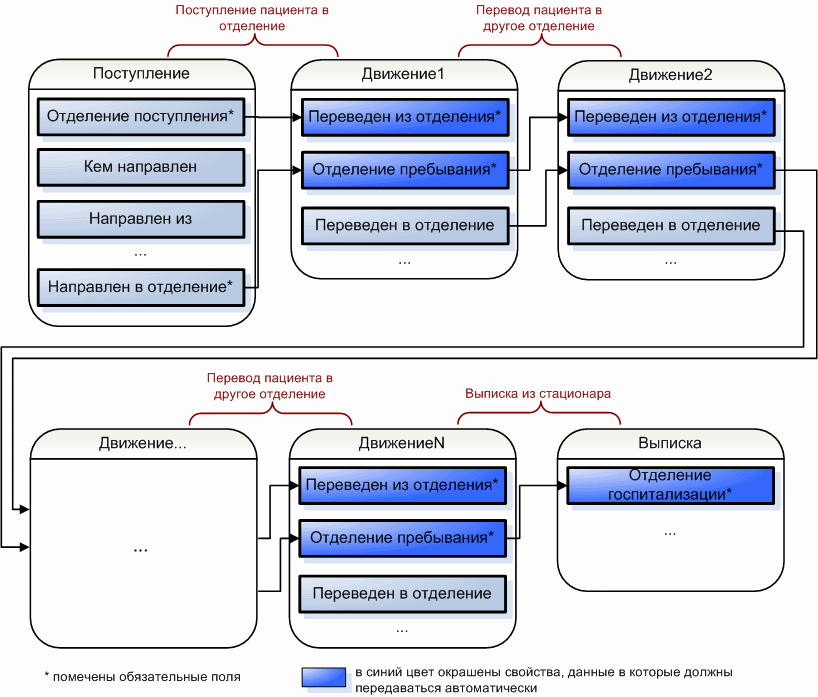
\includegraphics[width = 1\textwidth ,keepaspectratio]{spr_ln_dv}
 \caption{Схема автоматического заполнения полей в действиях группы <<Стационар>>}
 \label{img_spr_ln_dv}
\end{figure}

\begin{vnim}
Корректная настройка движения в стационаре особенно необходима при организации взаимодействия с <<1С: Аптека>>.
\end{vnim}

Для реализации данной схемы для типов действий <<Поступление>>, <<Движение>>, <<Выписка>> в поле \dm{Код для отчетов} должны быть указаны значения представленные в поле <<Мнемоника>> таблицы 15. Далее необходимо отредактировать (а при их отсутствии добавить) некоторые свойства перечисленных типов действий в соответствии с таблицей \ref{tbl_spr_dv_prop}.

\clearpage
{\small
\begin{longtable}{|p{3cm}|p{3.5cm}|p{2.8cm}|p{2cm}|p{2.2cm}|p{1cm}|p{1cm}|}
 \caption{Необходимые настройки свойств типов действий группы <<Стационар>> \label{tbl_spr_dv_prop}} \\
 \hline \rule{0pt}{15pt} \centering \textbf{Наименование} & \centering \textbf{Описание} & \centering \textbf{Тип} & \centering \textbf{Область} & \centering \textbf{Код} & \centering \textbf{Обя\-за\-тель\-ное} & \textbf{Толь\-ко для чтения} \\ \hline
 \endfirsthead
 \hline \rule{0pt}{15pt} \centering \textbf{Наименование} & \centering \textbf{Описание} & \centering \textbf{Тип} & \centering \textbf{Область} & \centering \textbf{Код} & \centering \textbf{Обя\-за\-тель\-ное} & \textbf{Толь\-ко для чтения} \\ \hline
 \endhead
  \multicolumn{7}{|l|}{\textbf{Поступление}} \\ \hline
  Отделение поступления	& Куда поступил \footnote{По умолчанию в поле указывается подразделение по умолчанию для данного рабочего места (и пользователя). Настройка данного параметра производится через меню \mm{Настройки \str Умолчания} в поле \dm{Подразделение}.} & 	OrgStructure & 	& OrgStruct Stay &	Да & \\ \hline	
  Кем направлен	& Наименование направившего МУ	& String & 'Поликли ника’, ‘аббревиатура наименования ЛПУ’, ‘Самообращение’, ‘Переведен из’ & & & \\ \hline			
  Направлен из	& Отделение из предыдущей ИБ \footnote{Данное поле требуется заполнять, если в поле \dm{Кем направлен} выбрано значение <<аббревиатура наименования ЛПУ>>. Тогда здесь следует выбрать подразделение ЛПУ из дерева структуры ЛПУ.}& OrgStructure &	&	OrgStruct Directed From & & \\ \hline		
  Направлен в отделение	& Отделение первоначальной госпитализации	& OrgStructure	& &	OrgStruct Direction & Да & \\ \hline	
  \multicolumn{7}{|l|}{\textbf{Движение}} \\ \hline	
  Переведен из отделения &	Из какого отделения поступил &	OrgStructure &	&	OrgStruct Received &	Да &	Да \\ \hline	
  Отделение пребывания	& Текущее отделение & OrgStructure	& & OrgStruct Stay	& Да &	Да \\ \hline	
  Переведен в отделение	& Отделение выбытия & 	OrgStructure & &	OrgStruct Transfer & & \\ \hline			
   \multicolumn{7}{|l|}{\textbf{Выписка}}  \\ \hline
  Отделение госпитализации &	Текущее отделение &	OrgStructure & &		HospOrg Struct &	Да &	Да \\ \hline  
\end{longtable}
} 

\begin{vnim}
Если происходит закрытие движения, после которого следует Выписка, по поле \dm{Переведен в отделение} НЕ должно заполняться ни при каких условиях
\end{vnim}

\subsection{Предопределенные значения кодов некоторых справочников}

Значения кодов справочника \dm{Типы обращений} приведены в таблице \ref{tbl_spr_tpobr_kod}.

{\small
\begin{table}[ht!]
\topcaption{Стандартные коды для типов обращений} \label{tbl_spr_tpobr_kod} 
 \begin{tabular}{|p{2cm}|p{4cm}|p{10.5cm}|}
  \hline \rule{0pt}{15pt} \centering \textbf{Код} & \centering \textbf{Название} & \hfil \textbf{Описание} \\ \hline
  4	& Диагностика	& Регистрация амбулаторных обращений пациентов с целью проведения диагностических исследований  \\ \hline
  5	& Диспансеризация	& Регистрация амбулаторных обращений пациентов для диспансеризации \\ \hline
  6	& Консультативный	& Регистрация амбулаторных обращений пациентов с целью получения консультации врача-специалиста \\ \hline
  clinic	& Дневной стационар	& Регистрация госпитализаций пациентов в дневной стационар. В обращении используется мастер закрытия \\ \hline
  hospital	& Круглосуточный стационар &	Регистрация госпитализаций пациентов в круглосуточный стационар. В обращении используется мастер закрытия \\ \hline
  policlinic	& Поликлиника	& Регистрация стандартных поликлинических (амбулаторных) обращений пациентов  \\ \hline
  stationary	& Стационар	& Регистрация госпитализаций пациентов в стационары всех типов (дневной, круглосуточный). В обращении НЕ используется мастер закрытия \\ \hline  
 \end{tabular}
\end{table}
}

Значения кодов справочника \dm{Тип полиса} приведены в таблице \ref{tbl_spr_polis_kod}.

{\small
\begin{table}[ht!]
\topcaption{Стандартные коды для типов полисов} \label{tbl_spr_polis_kod} 
 \begin{tabular}{|p{4.3 cm}|p{4.4cm}|p{7.9cm}|}
  \hline \rule{0pt}{15pt} \centering \textbf{Код} & \centering \textbf{Название} & \hfil \textbf{Описание} \\ \hline
  cmiOld &	Полис ОМС старого образца	& При вводе полиса в регистрационную карточку пациента требуется ввод серии и номера документа \\ \hline
  cmiTmp &	Временное свидетельство ОМС	& При вводе полиса в регистрационную карточку пациента требуется ввод серии и номера документа \\ \hline
  cmiCommonPaper &	Бумажный полис ОМС единого образца & 	При вводе полиса в регистрационную карточку пациента требуется ввод только номера документа \\ \hline
  cmiCommonElectron	& Электронный полис ОМС единого образца	& При вводе полиса в регистрационную карточку пациента требуется ввод только номера документа \\ \hline
  cmiUEC	& Полис ОМС в составе универсальной электронной карты (УЭК) & При вводе полиса в регистрационную карточку пациента требуется ввод серии и номера документа \\ \hline
  vmi	& Полис ДМС	& При вводе полиса в регистрационную карточку пациента требуется ввод серии и номера документа \\ \hline
  cmiFnkcIndustrial	& Полис ОМС Производственный & Оставлен для совместимости со старой версией системы \\ \hline
  cmiFnkcLocal	& Полис ОМС Территориальный	& Оставлен для совместимости со старой версией системы \\ \hline
 \end{tabular}
\end{table}
}

Значения кодов справочника \dm{Типы действий} для идентификации некоторых элементов данного справочника приведены в таблице \ref{tbl_spr_tpact_kod}.

{\small
\begin{table}
\topcaption{Стандартные коды типов действий} \label{tbl_spr_tpact_kod} 
 \begin{tabular}{|p{1.5 cm}|p{3cm}|p{12.2cm}|}
  \hline \rule{0pt}{15pt} \centering \textbf{Код} & \centering \textbf{Мнемоника} & \hfil \textbf{Тип действия} \\ \hline
  4201 &	received	& Поступление пациента (для госпитализации) \\ \hline 
  4202 &	moving	& Движение пациента (в стационаре) \\ \hline
  4203	& leaved	& Выписка пациента из стационара \\ \hline
  4504	& & Заключительный эпикриз  \\ \hline
  4507	& & Посмертный эпикриз  \\ \hline
  	& del\_received	& Отмена предыдущего сообщения о госпитализации \\ \hline
  	& del\_moving &	Отмена предыдущего сообщения о переводе пациента между отделениями внутри стационара  \\ \hline
  	& prescription &	Терапия (Медикаментозное назначение) \\ \hline
  	& infusion	& Инфузионная терапия (Медикаментозное назначение) \\ \hline
  	& chemotherapy	& Химиотерапия (Медикаментозное назначение) \\ \hline
  	& analgesia	& Анальгезия (Медикаментозное назначение) \\ \hline
 \end{tabular}
\end{table}
}

\begin{vnim}
Нельзя присваивать нескольким типам действий один и тот же код. Значения кода должны быть уникальны в БД.
\end{vnim}

Значения кодов справочника \dm{Группа типа документа (удостоверения, льготы и т.д.)} приведены в таблице \ref{tbl_spr_grdoc_kod}.

{\small
\begin{table}
\topcaption{Стандартные коды групп типов документов} \label{tbl_spr_grdoc_kod} 
 \begin{tabular}{|p{2 cm}|p{15cm}|}
  \hline \rule{0pt}{15pt} \centering \textbf{Код} & \hfil \textbf{Название} \\ \hline
  1	& Удостоверение личности  \\ \hline
  2	& Льготы \\ \hline
  5	& Риски \\ \hline
  7	& Инвалидность \\ \hline
 \end{tabular}
\end{table}
}

